% Options for packages loaded elsewhere
% Options for packages loaded elsewhere
\PassOptionsToPackage{unicode}{hyperref}
\PassOptionsToPackage{hyphens}{url}
%
\documentclass[
  ignorenonframetext,
  aspectratio=169,
]{beamer}
\newif\ifbibliography
\usepackage{pgfpages}
\setbeamertemplate{caption}[numbered]
\setbeamertemplate{caption label separator}{: }
\setbeamercolor{caption name}{fg=normal text.fg}
\beamertemplatenavigationsymbolsempty
% remove section numbering
\setbeamertemplate{part page}{
  \centering
  \begin{beamercolorbox}[sep=16pt,center]{part title}
    \usebeamerfont{part title}\insertpart\par
  \end{beamercolorbox}
}
\setbeamertemplate{section page}{
  \centering
  \begin{beamercolorbox}[sep=12pt,center]{section title}
    \usebeamerfont{section title}\insertsection\par
  \end{beamercolorbox}
}
\setbeamertemplate{subsection page}{
  \centering
  \begin{beamercolorbox}[sep=8pt,center]{subsection title}
    \usebeamerfont{subsection title}\insertsubsection\par
  \end{beamercolorbox}
}
% Prevent slide breaks in the middle of a paragraph
\widowpenalties 1 10000
\raggedbottom
\AtBeginPart{
  \frame{\partpage}
}
\AtBeginSection{
  \ifbibliography
  \else
    \frame{\sectionpage}
  \fi
}
\AtBeginSubsection{
  \frame{\subsectionpage}
}
\usepackage{iftex}
\ifPDFTeX
  \usepackage[T1]{fontenc}
  \usepackage[utf8]{inputenc}
  \usepackage{textcomp} % provide euro and other symbols
\else % if luatex or xetex
  \usepackage{unicode-math} % this also loads fontspec
  \defaultfontfeatures{Scale=MatchLowercase}
  \defaultfontfeatures[\rmfamily]{Ligatures=TeX,Scale=1}
\fi
\usepackage{lmodern}

\ifPDFTeX\else
  % xetex/luatex font selection
\fi
% Use upquote if available, for straight quotes in verbatim environments
\IfFileExists{upquote.sty}{\usepackage{upquote}}{}
\IfFileExists{microtype.sty}{% use microtype if available
  \usepackage[]{microtype}
  \UseMicrotypeSet[protrusion]{basicmath} % disable protrusion for tt fonts
}{}
\makeatletter
\@ifundefined{KOMAClassName}{% if non-KOMA class
  \IfFileExists{parskip.sty}{%
    \usepackage{parskip}
  }{% else
    \setlength{\parindent}{0pt}
    \setlength{\parskip}{6pt plus 2pt minus 1pt}}
}{% if KOMA class
  \KOMAoptions{parskip=half}}
\makeatother

\usepackage{color}
\usepackage{fancyvrb}
\newcommand{\VerbBar}{|}
\newcommand{\VERB}{\Verb[commandchars=\\\{\}]}
\DefineVerbatimEnvironment{Highlighting}{Verbatim}{commandchars=\\\{\}}
% Add ',fontsize=\small' for more characters per line
\usepackage{framed}
\definecolor{shadecolor}{RGB}{241,243,245}
\newenvironment{Shaded}{\begin{snugshade}}{\end{snugshade}}
\newcommand{\AlertTok}[1]{\textcolor[rgb]{0.68,0.00,0.00}{#1}}
\newcommand{\AnnotationTok}[1]{\textcolor[rgb]{0.37,0.37,0.37}{#1}}
\newcommand{\AttributeTok}[1]{\textcolor[rgb]{0.40,0.45,0.13}{#1}}
\newcommand{\BaseNTok}[1]{\textcolor[rgb]{0.68,0.00,0.00}{#1}}
\newcommand{\BuiltInTok}[1]{\textcolor[rgb]{0.00,0.23,0.31}{#1}}
\newcommand{\CharTok}[1]{\textcolor[rgb]{0.13,0.47,0.30}{#1}}
\newcommand{\CommentTok}[1]{\textcolor[rgb]{0.37,0.37,0.37}{#1}}
\newcommand{\CommentVarTok}[1]{\textcolor[rgb]{0.37,0.37,0.37}{\textit{#1}}}
\newcommand{\ConstantTok}[1]{\textcolor[rgb]{0.56,0.35,0.01}{#1}}
\newcommand{\ControlFlowTok}[1]{\textcolor[rgb]{0.00,0.23,0.31}{\textbf{#1}}}
\newcommand{\DataTypeTok}[1]{\textcolor[rgb]{0.68,0.00,0.00}{#1}}
\newcommand{\DecValTok}[1]{\textcolor[rgb]{0.68,0.00,0.00}{#1}}
\newcommand{\DocumentationTok}[1]{\textcolor[rgb]{0.37,0.37,0.37}{\textit{#1}}}
\newcommand{\ErrorTok}[1]{\textcolor[rgb]{0.68,0.00,0.00}{#1}}
\newcommand{\ExtensionTok}[1]{\textcolor[rgb]{0.00,0.23,0.31}{#1}}
\newcommand{\FloatTok}[1]{\textcolor[rgb]{0.68,0.00,0.00}{#1}}
\newcommand{\FunctionTok}[1]{\textcolor[rgb]{0.28,0.35,0.67}{#1}}
\newcommand{\ImportTok}[1]{\textcolor[rgb]{0.00,0.46,0.62}{#1}}
\newcommand{\InformationTok}[1]{\textcolor[rgb]{0.37,0.37,0.37}{#1}}
\newcommand{\KeywordTok}[1]{\textcolor[rgb]{0.00,0.23,0.31}{\textbf{#1}}}
\newcommand{\NormalTok}[1]{\textcolor[rgb]{0.00,0.23,0.31}{#1}}
\newcommand{\OperatorTok}[1]{\textcolor[rgb]{0.37,0.37,0.37}{#1}}
\newcommand{\OtherTok}[1]{\textcolor[rgb]{0.00,0.23,0.31}{#1}}
\newcommand{\PreprocessorTok}[1]{\textcolor[rgb]{0.68,0.00,0.00}{#1}}
\newcommand{\RegionMarkerTok}[1]{\textcolor[rgb]{0.00,0.23,0.31}{#1}}
\newcommand{\SpecialCharTok}[1]{\textcolor[rgb]{0.37,0.37,0.37}{#1}}
\newcommand{\SpecialStringTok}[1]{\textcolor[rgb]{0.13,0.47,0.30}{#1}}
\newcommand{\StringTok}[1]{\textcolor[rgb]{0.13,0.47,0.30}{#1}}
\newcommand{\VariableTok}[1]{\textcolor[rgb]{0.07,0.07,0.07}{#1}}
\newcommand{\VerbatimStringTok}[1]{\textcolor[rgb]{0.13,0.47,0.30}{#1}}
\newcommand{\WarningTok}[1]{\textcolor[rgb]{0.37,0.37,0.37}{\textit{#1}}}

\usepackage{longtable,booktabs,array}
\newcounter{none} % for unnumbered tables
\usepackage{calc} % for calculating minipage widths
\usepackage{caption}
% Make caption package work with longtable
\makeatletter
\def\fnum@table{\tablename~\thetable}
\makeatother
\usepackage{graphicx}
\makeatletter
\newsavebox\pandoc@box
\newcommand*\pandocbounded[1]{% scales image to fit in text height/width
  \sbox\pandoc@box{#1}%
  \Gscale@div\@tempa{\textheight}{\dimexpr\ht\pandoc@box+\dp\pandoc@box\relax}%
  \Gscale@div\@tempb{\linewidth}{\wd\pandoc@box}%
  \ifdim\@tempb\p@<\@tempa\p@\let\@tempa\@tempb\fi% select the smaller of both
  \ifdim\@tempa\p@<\p@\scalebox{\@tempa}{\usebox\pandoc@box}%
  \else\usebox{\pandoc@box}%
  \fi%
}
% Set default figure placement to htbp
\def\fps@figure{htbp}
\makeatother





\setlength{\emergencystretch}{3em} % prevent overfull lines

\providecommand{\tightlist}{%
  \setlength{\itemsep}{0pt}\setlength{\parskip}{0pt}}



 


\setbeamertemplate{frametitle continuation}{}
\setbeamertemplate{itemize items}[circle]
\usepackage{caption}
\captionsetup{labelformat=empty, justification=centering}
\usepackage{textpos}
\setlength{\TPHorizModule}{1cm}
\setlength{\TPVertModule}{1cm}
\setbeamertemplate{footline}{%
  \hfill\usebeamercolor[fg]{page number in head/foot}%
  \usebeamerfont{page number in head/foot}%
  \insertframenumber{} / \inserttotalframenumber\kern1em\vskip2pt%
}
\usepackage{xcolor}
\let\oldtexttt\texttt
\renewcommand{\texttt}[1]{\colorbox{gray!20}{\oldtexttt{#1}}}

% highlights
\definecolor{bluebeamer}{HTML}{3333B3}
\newcommand{\bluenorm}[1]{\textcolor{bluebeamer}{#1}}
\newcommand{\blueit}[1]{\textcolor{bluebeamer}{\emph{#1}}}
\newcommand{\bluebold}[1]{\textcolor{bluebeamer}{\textbf{#1}}}
\makeatletter
\@ifpackageloaded{caption}{}{\usepackage{caption}}
\AtBeginDocument{%
\ifdefined\contentsname
  \renewcommand*\contentsname{Table of contents}
\else
  \newcommand\contentsname{Table of contents}
\fi
\ifdefined\listfigurename
  \renewcommand*\listfigurename{List of Figures}
\else
  \newcommand\listfigurename{List of Figures}
\fi
\ifdefined\listtablename
  \renewcommand*\listtablename{List of Tables}
\else
  \newcommand\listtablename{List of Tables}
\fi
\ifdefined\figurename
  \renewcommand*\figurename{Figure}
\else
  \newcommand\figurename{Figure}
\fi
\ifdefined\tablename
  \renewcommand*\tablename{Table}
\else
  \newcommand\tablename{Table}
\fi
}
\@ifpackageloaded{float}{}{\usepackage{float}}
\floatstyle{ruled}
\@ifundefined{c@chapter}{\newfloat{codelisting}{h}{lop}}{\newfloat{codelisting}{h}{lop}[chapter]}
\floatname{codelisting}{Listing}
\newcommand*\listoflistings{\listof{codelisting}{List of Listings}}
\makeatother
\makeatletter
\makeatother
\makeatletter
\@ifpackageloaded{caption}{}{\usepackage{caption}}
\@ifpackageloaded{subcaption}{}{\usepackage{subcaption}}
\makeatother

\usepackage{bookmark}
\IfFileExists{xurl.sty}{\usepackage{xurl}}{} % add URL line breaks if available
\urlstyle{same}
% fallback for those not using the hyperref driver hyperxmp:
\makeatletter
\@ifundefined{xmpquote}{\newcommand{\xmpquote}[1]{#1}}{}
\makeatother
\hypersetup{
  pdftitle={Introduction to Basic and Advanced Statistical Modelling},
  pdfauthor={Alexandre Courtiol},
  hidelinks,
  pdfcreator={LaTeX via pandoc}}


\title{\texorpdfstring{Introduction to Basic and Advanced Statistical
Modelling}{Introduction to Basic and Advanced Statistical Modelling}}
\subtitle{\texorpdfstring{Using R}{Using R}}
\author{Alexandre Courtiol}
\date{}

\begin{document}
\frame{\titlepage}

\renewcommand*\contentsname{Table of contents}
\begin{frame}[allowframebreaks]
  \frametitle{Table of contents}
  \setcounter{tocdepth}{3}
  \tableofcontents
\end{frame}
\setcounter{tocdepth}{3}
\tableofcontents
}

\section{RStudio}\label{rstudio}

\begin{frame}{Installation}
\protect\phantomsection\label{installation}
\begin{itemize}
\tightlist
\item
  install R: \url{https://cran.r-project.org/}
\item
  install RStudio Desktop:
  \url{https://posit.co/download/rstudio-desktop/}
\item
  let us set the global options properly together
\end{itemize}
\end{frame}

\begin{frame}{RStudio panes}
\protect\phantomsection\label{rstudio-panes}
\footnotesize

\begin{center}
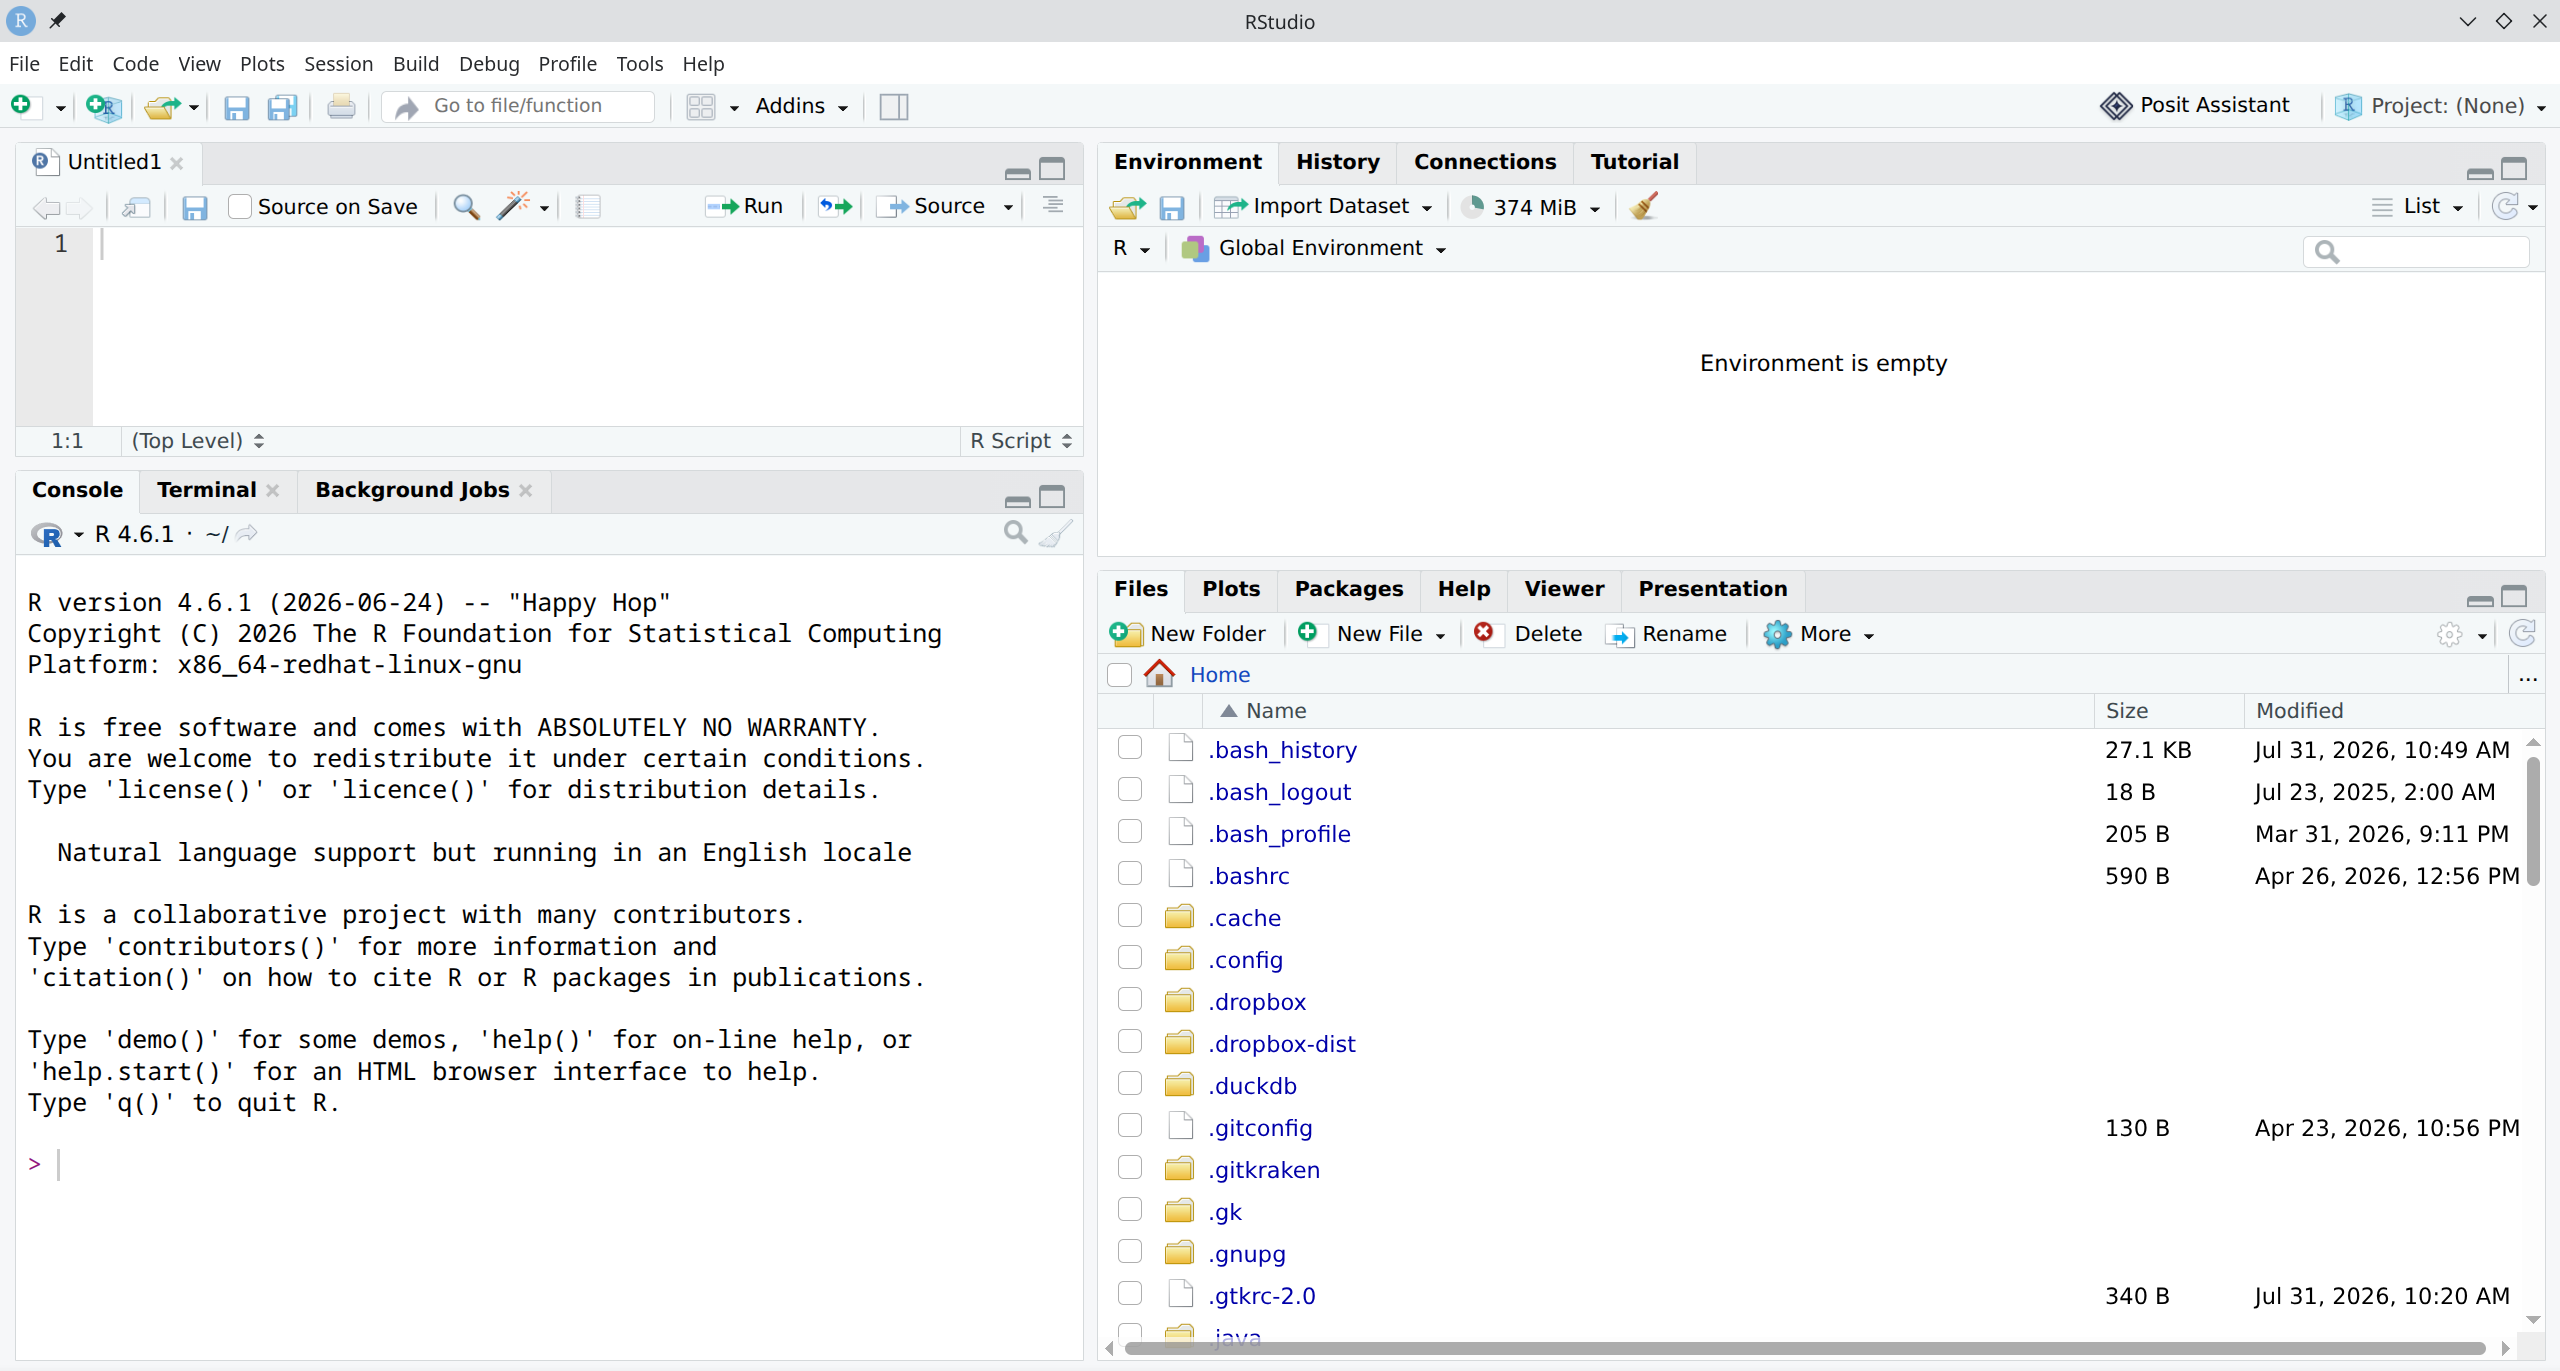
\includegraphics[width=\linewidth,height=10cm,keepaspectratio]{figures/Rstudio.png}
\end{center}

\normalsize
\end{frame}

\begin{frame}{Practice 1}
\protect\phantomsection\label{practice-1}
Let's setup our working environment:

\begin{enumerate}
\tightlist
\item
  create a new project
\item
  create a new R script
\item
  save the created R script into the project folder directory
\end{enumerate}

\vfill

\textbf{NB:}

\begin{itemize}
\tightlist
\item
  a project is defined by a simple (text) file. Its main benefit is to
  open RStudio with the correct working directory set (that is, the one
  where the project file is)
\item
  an R script is a (text) file where we can write R code
\end{itemize}
\end{frame}

\begin{frame}{Practice 2}
\protect\phantomsection\label{practice-2}
Let's install the following R packages:

\begin{enumerate}
\tightlist
\item
  \{tidyverse\}
\item
  \{sf\}
\end{enumerate}

\vfill

\textbf{NB:}

\begin{itemize}
\tightlist
\item
  I will try to use \{\} consistently to indicate that something is a
  package
\item
  installing a package is only required once, unless you want to update
  the package or unless you installed a new version of R
\item
  I recommend using RStudio for installing packages to avoid running the
  installation code every time you restart your session
\end{itemize}
\end{frame}

\section{Reading data}\label{reading-data}

\begin{frame}{The datasets}
\protect\phantomsection\label{the-datasets}
\footnotesize

\begin{center}

\includegraphics[width=\linewidth,height=4cm,keepaspectratio]{figures/MHB.png}
\end{center}

\normalsize

\vspace{1em}

\begin{quote}
Since 1999, 267 one-km squares laid out in a mostly systematic grid
across all of Switzerland have been surveyed annually by skilled, mostly
volunteer ornithologists. Bird populations are recorded using a
simplified territory mapping protocol with two visits per square above
the timberline and three elsewhere. Surveys are conducted during the
breeding season (mid-April to early July) along a square-specific
transect route that does not change over the years.
\end{quote}
\end{frame}

\begin{frame}[fragile]{Practice 3}
\protect\phantomsection\label{practice-3}
\begin{enumerate}
\tightlist
\item
  download the datasets from the following location:
  \url{https://zenodo.org/records/18480886}
\item
  extract the datasets into your R project within a folder called
  data\_MHB
\end{enumerate}

\pause

\vspace{1cm}

\textbf{Pro tips:}

\begin{itemize}
\tightlist
\item
  you can use \texttt{getwd()} to check where your project folder is
  located
\item
  this could be done using R code, but it is not necessary, nor useful
  here
\end{itemize}
\end{frame}

\begin{frame}[fragile]{Activating the \{tidyverse\}}
\protect\phantomsection\label{activating-the-tidyverse}
\footnotesize

\begin{Shaded}
\begin{Highlighting}[]
\FunctionTok{library}\NormalTok{(tidyverse)}
\end{Highlighting}
\end{Shaded}

\begin{verbatim}
-- Attaching core tidyverse packages ---------------------------------- tidyverse 2.0.0 --
v dplyr     1.2.1     v readr     2.2.0
v forcats   1.0.1     v stringr   1.6.0
v ggplot2   4.0.3     v tibble    3.3.1
v lubridate 1.9.5     v tidyr     1.3.2
v purrr     1.2.2     
-- Conflicts ---------------------------------------------------- tidyverse_conflicts() --
x dplyr::filter() masks stats::filter()
x dplyr::lag()    masks stats::lag()
i Use the conflicted package (<http://conflicted.r-lib.org/>) to force all conflicts to become errors
\end{verbatim}

\normalsize
\end{frame}

\begin{frame}{The \{tidyverse\} environment}
\protect\phantomsection\label{the-tidyverse-environment}
The \{tidyverse\} is a meta package encapsulating an ecosystem of R
packages (see \url{https://www.tidyverse.org} for more).

\vspace{1em}

There are currently 9 core packages automatically attached by the
\{tidyverse\}:

\begin{center}
\raisebox{-0.5\height}{\includegraphics[width = 1.5cm]{"figures/tidyverse/hex-tidyverse"}}
=
\raisebox{-0.5\height}{\includegraphics[width = 1cm]{"figures/tidyverse/hex-tibble"}}
\raisebox{-0.5\height}{\includegraphics[width = 1cm]{"figures/tidyverse/hex-readr"}}
\raisebox{-0.5\height}{\includegraphics[width = 1cm]{"figures/tidyverse/hex-dplyr"}}
\raisebox{-0.5\height}{\includegraphics[width = 1cm]{"figures/tidyverse/hex-stringr"}}
\raisebox{-0.5\height}{\includegraphics[width = 1cm]{"figures/tidyverse/hex-lubridate"}}
\raisebox{-0.5\height}{\includegraphics[width = 1cm]{"figures/tidyverse/hex-forcats"}}
\raisebox{-0.5\height}{\includegraphics[width = 1cm]{"figures/tidyverse/hex-tidyr"}}
\raisebox{-0.5\height}{\includegraphics[width = 1cm]{"figures/tidyverse/hex-ggplot2"}}
\raisebox{-0.5\height}{\includegraphics[width = 1cm]{"figures/tidyverse/hex-purrr"}}
\end{center}

\vfill

\begin{itemize}
\tightlist
\item
  philosophy: making R more accessible
\item
  backward compatibility is not strictly enforced
\end{itemize}
\end{frame}

\begin{frame}[fragile]{Let's import the first dataset}
\protect\phantomsection\label{lets-import-the-first-dataset}
\footnotesize

\begin{Shaded}
\begin{Highlighting}[]
\NormalTok{species\_count }\OtherTok{\textless{}{-}} \FunctionTok{read\_csv}\NormalTok{(}\StringTok{"data\_MHB/header{-}species{-}count.csv"}\NormalTok{)}
\end{Highlighting}
\end{Shaded}

\begin{verbatim}
Rows: 7113 Columns: 10
-- Column specification ------------------------------------------------------------------
Delimiter: ","
dbl (10): samplearea_id, x-koord, y-koord, lon, lat, year, route_length, median_elevat...

i Use `spec()` to retrieve the full column specification for this data.
i Specify the column types or set `show_col_types = FALSE` to quiet this message.
\end{verbatim}

\normalsize
\end{frame}

\begin{frame}[fragile]{Let's check the first dataset}
\protect\phantomsection\label{lets-check-the-first-dataset}
\footnotesize

\begin{Shaded}
\begin{Highlighting}[]
\NormalTok{species\_count}
\end{Highlighting}
\end{Shaded}

\begin{verbatim}
# A tibble: 7,113 x 10
  samplearea_id `x-koord` `y-koord`   lon   lat  year route_length median_elevation
          <dbl>     <dbl>     <dbl> <dbl> <dbl> <dbl>        <dbl>            <dbl>
1           268   2725500   1182500  9.08  46.8  1999         4444             1550
2           268   2725500   1182500  9.08  46.8  2000         4444             1550
3           268   2725500   1182500  9.08  46.8  2001         4444             1550
# i 7,110 more rows
# i 2 more variables: n_visits <dbl>, n_recorded_species <dbl>
\end{verbatim}

\normalsize

\pause

\textbf{Pro tips:}

\begin{itemize}
\tightlist
\item
  check the output (a tibble) carefully to make sure you read in your
  data properly
\item
  if your are not using \{readr\}, the output may not be a tibble and
  would be better checked using \texttt{str()}
\end{itemize}
\end{frame}

\begin{frame}[fragile]{Practice 4}
\protect\phantomsection\label{practice-4}
\begin{itemize}
\tightlist
\item
  import the file \texttt{data-territories.csv} to obtain the second
  dataset
\end{itemize}

\footnotesize

\normalsize

\footnotesize

\begin{Shaded}
\begin{Highlighting}[]
\NormalTok{territories}
\end{Highlighting}
\end{Shaded}

\begin{verbatim}
# A tibble: 1,152,306 x 10
  species_id euring_id nameeg       namelt         samplearea_id  year territories_visit_1
       <dbl>     <dbl> <chr>        <chr>                  <dbl> <dbl>               <dbl>
1         50        70 Little Grebe Tachybaptus r~           268  1999                   0
2         50        70 Little Grebe Tachybaptus r~           268  2000                   0
3         50        70 Little Grebe Tachybaptus r~           268  2001                   0
# i 1,152,303 more rows
# i 3 more variables: territories_visit_2 <dbl>, territories_visit_3 <dbl>,
#   territories_total <dbl>
\end{verbatim}

\normalsize

\pause

\textbf{Pro tips:}

\begin{itemize}
\tightlist
\item
  use \texttt{View()} to explore the datasets in an Excel-like fashion
\end{itemize}
\end{frame}

\section{Wrangling data}\label{wrangling-data}

\begin{frame}{Data wrangling with \{dplyr\}}
\protect\phantomsection\label{data-wrangling-with-dplyr}
In \{dplyr\} much can be achieved with a few functions

\footnotesize

\begin{center}
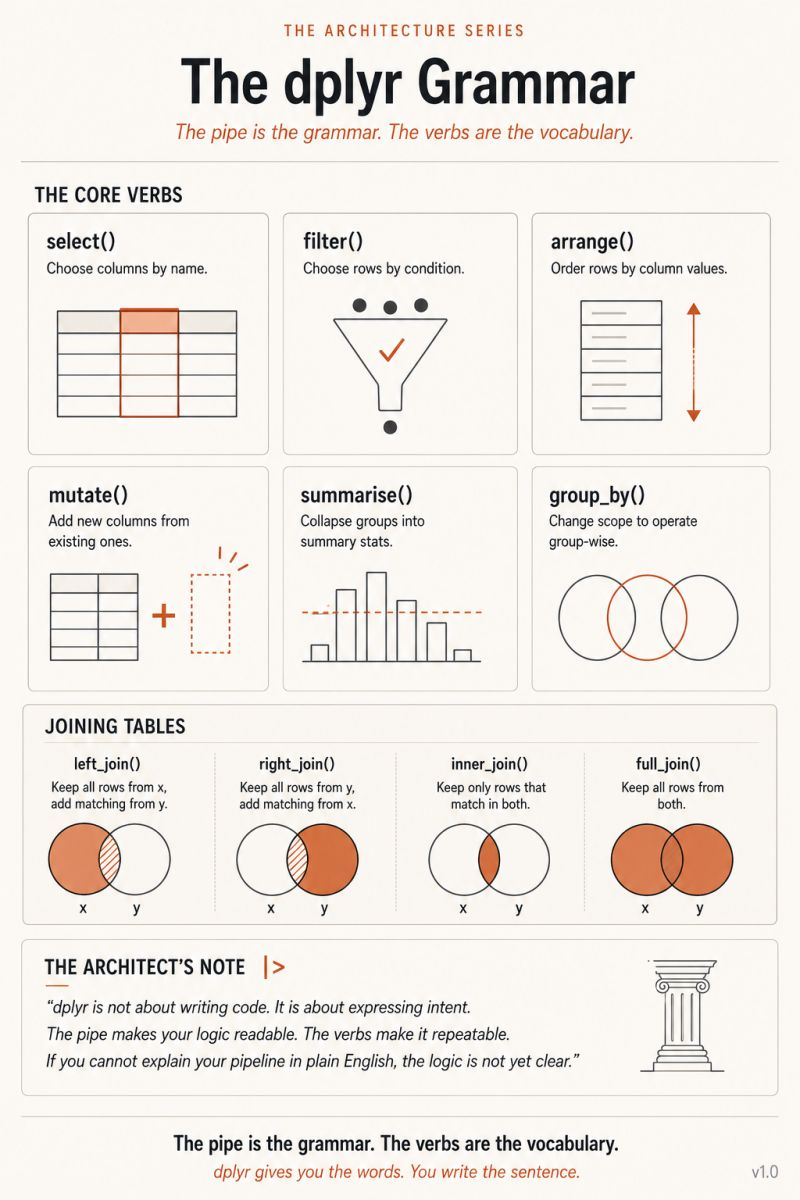
\includegraphics[width=\linewidth,height=5cm,keepaspectratio]{figures/dplyr.jpg}
\end{center}

\normalsize

\begin{center}
\begingroup \tiny source: \url{https://linkedin.com/in/adalbert-ngongang-phd-637995a3}\endgroup
\end{center}

We will study some of these functions and a few others to get you going
\end{frame}

\begin{frame}[fragile]{Choose columns using \texttt{select()}}
\protect\phantomsection\label{choose-columns-using-select}
\footnotesize

\begin{Shaded}
\begin{Highlighting}[]
\NormalTok{species\_count }\SpecialCharTok{|\textgreater{}} \FunctionTok{select}\NormalTok{(samplearea\_id, year, n\_recorded\_species)}
\end{Highlighting}
\end{Shaded}

\begin{verbatim}
# A tibble: 7,113 x 3
  samplearea_id  year n_recorded_species
          <dbl> <dbl>              <dbl>
1           268  1999                 27
2           268  2000                 25
3           268  2001                 30
# i 7,110 more rows
\end{verbatim}

\normalsize

\pause

\textbf{Pro tips:}

\begin{itemize}
\tightlist
\item
  you can use \texttt{-column\_name} to drop a column called
  \texttt{column\_name}
\item
  you can use selection helpers (e.g.~\texttt{contains()},
  \texttt{starts\_with()}) to select columns using name patterns
\item
  you can use test(s) on column values to select them (\texttt{where()})
\end{itemize}
\end{frame}

\begin{frame}[fragile]{A few words about the pipe
\texttt{\textbar{}\textgreater{}}}
\protect\phantomsection\label{a-few-words-about-the-pipe}
\footnotesize

\begin{Shaded}
\begin{Highlighting}[]
\NormalTok{species\_count }\SpecialCharTok{|\textgreater{}} \FunctionTok{select}\NormalTok{(samplearea\_id, year, n\_recorded\_species)}
\end{Highlighting}
\end{Shaded}

\normalsize

is interpreted exactly as this:

\footnotesize

\begin{Shaded}
\begin{Highlighting}[]
\FunctionTok{select}\NormalTok{(species\_count, samplearea\_id, year, n\_recorded\_species)}
\end{Highlighting}
\end{Shaded}

\normalsize

\textbf{NB:}

\begin{itemize}
\tightlist
\item
  the pipe captures what precedes it and considers it as the first
  argument of the function that follows it
\item
  it makes the code more readable, as it emphasises the sequence of
  operations applied to the data
\end{itemize}
\end{frame}

\begin{frame}[fragile]{Extract one column using \texttt{pull()}}
\protect\phantomsection\label{extract-one-column-using-pull}
You can use \texttt{select()} to choose one column, but it will remain a
table (technically an object of class \texttt{tibble} or
\texttt{data.frame}):

\footnotesize

\begin{Shaded}
\begin{Highlighting}[]
\NormalTok{species\_count }\SpecialCharTok{|\textgreater{}} \FunctionTok{select}\NormalTok{(n\_recorded\_species)}
\end{Highlighting}
\end{Shaded}

\begin{verbatim}
# A tibble: 7,113 x 1
  n_recorded_species
               <dbl>
1                 27
2                 25
3                 30
# i 7,110 more rows
\end{verbatim}

\normalsize

\pause

Instead \texttt{pull()} creates a vector, which can be easier to work
with:

\footnotesize

\begin{Shaded}
\begin{Highlighting}[]
\NormalTok{species\_count }\SpecialCharTok{|\textgreater{}} \FunctionTok{pull}\NormalTok{(n\_recorded\_species)}
\end{Highlighting}
\end{Shaded}

\begin{verbatim}
   [1] 27 25 30 31 29 29 38 27 29 39 30 37 44 36 37 33 35 34 42 31 42 33 37 31 32 33 42 29
  [29] 28 32 28 30 29 26 28 29 31 37 30 27 28 27 30 26 30 27 29 29 29 26 29 28 25 27 37 37
  [57] 42 46 42 41 40 41 40 42 40 45 42 41 44 40 36 34 37 36 39 43 45 41 42 44 43 38 32 34
  [85] 32 37 37 34 34 33 33 33 37 32 34 31 32 32 33 36 35 36 54 39 44 45 42 39 34 37 33 33
 [113] 33 43 41 41 37 34 42 36 39 37 34 37 40 34 38 37 36 37 39 36 31 34 30 39 41 46 42 46
 [141] 38 47 34 41 47 51 49 41 43 51 49 52 49 43 46 52 46 43 44 46 43 45 49 41 37 42 38 43
 [169] 42 42 42 40 44 44 43 43 41 41 41 37 41 43 39 44 42 38 41 43 48 47 48 42 43 40 42 48
 [197] 50 45 48 51 50 47 47 40 51 41 43 35 40 45 37 35 43 41 33 42 36 39 36 36 38 42 47 39
 [225] 42 37 38 41 38 46 43 40 36 42 40 44 40 40 38 36 39 38 37 39 39 37 30 35 41 36 38 40
 [253] 40 39 44 40 42 38 33 35 40 41 36 34 39 34 32 33 33 30 31 37 35 41 39 45 42 45 39 42
 [281] 39 40 44 42 42 34 42 40 39 37 35 36 35 34 44 46 34 40 40 47 40 42 39 40 36 37 38 41
 [309] 37 42 41 36 39 44 43 41 45 43 45 27 25 23 29 26 26 31 27 30 27 25 28 30 27 29 30 28
 [337] 42 40 28 31 37 37 40 32 32 35 36 39 38 39 30 30 36 29 33 34 34 33 34 31 32 37 35 40
 [365] 32 34 32 34 37 29 26 24 23 26 25 24 29 28 27 32 27 28 27 24 31 32 26 28 27 29 34 30
 [393] 34 42 37 32 27 31 44 38 44 42 45 41 41 41 40 31 31 33 37 35 36 44 35 41 37 44 48 43
 [421] 41 44 41 30 36 31 30 33 35 43 40 37 36 39 37 41 39 42 42 40 42 40 45 44 41 41 42 46
 [449] 42 35 33 36 36 37 41 39 44 38 37 30 34 33 27 40 35 35 39 30 41 43 42 40 35 42 39 43
 [477] 41 39 42 35 38 30 44 39 44 41 41 40 45 44 45 40 40 36 38 46 45 44 47 41 42 40 42 45
 [505] 46 51 48 47 44 41 46 47 46 43 40 44 44 46 42 48 42 45 39 38 38 38 37 38 35 37 26 23
 [533] 27 29 28 25 27 24 24 27 27 23 28 26 26 24 32 31 30 29 23 19 32 28 29 32 28 48 45 44
 [561] 43 43 43 45 46 48 39 44 45 44 45 43 38 37 40 37 45 38 43 37 38 49 42 40 32 32 43 40
 [589] 40 42 42 46 43 45 43 44 47 46 47 46 47 46 45 49 48 44 49 45 49 34 28 34 29 30 31 30
 [617] 28 31 32 32 30 31 35 40 37 34 31 39 35 39 41 42 41 42 45 42 35 41 37 40 36 41 41 43
 [645] 43 38 39 42 45 43 42 37 41 37 39 45 42 44 41 42 42 38 45 43 48 42 44 40 46 36 36 40
 [673] 45 45 45 40 38 46 43 44 43 43 40 50 47 38 42 47 45 33 36 35 26 29 28 28 39 41 42 39
 [701] 44 42 36 43 38 41 39 40 32 36 37 34 40 46 46 42 46 47 44 42 45 48 49 45 45 48 46 47
 [729] 43 45 46 44 42 49 40 48 50 51 44 51 45 50 44 41 41 39 37 37 36 38 45 45 43 40 44 35
 [757] 43 40 39 35 44 42 38 44 37 38 36 38 39 37 40 37 35 38 37 38 35 44 42 35 34 39 37 36
 [785] 38 35 38 30 32 41 39 33 34 37 35 36 44 47 53 47 52 51 52 50 49 48 48 48 52 42 42 46
 [813] 38 45 38 41 41 43 45 42 40 39 39 34 32 37 39 39 40 37 33 33 37 34 33 33 40 36 39 38
 [841] 34 36 36 44 42 47 47 44 38 43 29 33 30 33 39 34 33 33 32 32 32 35 36 39 31 34 32 36
 [869] 38 35 36 40 40 37 35 38 37 39 43 35 38 32 38 41 37 39 39 31 45 46 48 46 46 51 37 47
 [897] 50 47 50 51 47 46 49 46 44 38 41 31 41 27 42 37 43 36 38 40 35 44 36 45 40 43 41 36
 [925] 42 41 41 42 39 44 47 28 28 28 26 37 36 43 39 35 36 39 36 34 36 31 39 40 37 38 41 35
 [953] 39 37 32 38 37 30 35 30 40 29 32 25 35 31 37 36 33 36 36 31 39 40 36 29 26 32 32 33
 [981] 30 30 29 31 32 45 43 45 38 46 50 46 43 38 39 38 42 42 44 44 40 38 35 39 31 37 41 39
[1009] 38 37 39 42 40 38 31 38 37 34 40 48 46 41 48 48 45 51 44 48 44 49 50 50 47 49 48 47
[1037] 48 44 41 48 47 47 44 48 44 29 40 42 41 35 38 46 47 48 45 38 47 39 44 40 41 43 44 45
[1065] 44 33 41 35 43 39 42 41 40 38 41 41 42 38 40 41 34 41 43 43 35 38 42 47 49 44 40 44
[1093] 31 31 32 29 38 38 29 40 34 39 39 29 37 41 33 35 36 33 42 33 32 34 31 34 34 35 36 38
[1121] 31 38 38 43 38 39 36 40 41 43 47 27 35 38 42 41 39 40 46 47 43 43 42 44 27 28 28 30
[1149] 26 25 29 31 28 28 29 30 29 29 21 27 36 28 28 25 26 27 29 32 31 28 29 18 22 17 20 23
[1177] 21 22 21 20 23 22 24 25 21 17 25 23 20 26 26 18 24 26 24 29 19 25 43 45 44 45 48 49
[1205] 48 49 46 45 46 42 43 43 50 41 44 44 43 42 44 43 44 42 46 49 44 45 43 49 48 46 45 42
[1233] 43 40 43 43 43 45 40 42 43 41 43 37 37 34 44 33 44 46 51 45 26 28 32 27 29 27 28 27
[1261] 27 26 27 34 29 25 29 25 29 27 25 29 25 25 28 26 32 34 32 29 29 34 41 40 40 38 38 34
[1289] 29 34 40 35 37 38 32 35 42 35 37 39 39 38 35 36 37 32 12 18 13 18 12 15 14 18 14 16
[1317] 13 16 16 18 16 15 18 12 16 16 15 18 16 15 17 23 25 37 42 37 45 36 40 43 44 40 47 38
[1345] 42 39 40 41 41 46 43 43 39 45 45 43 45 46 42 44  8  7  9  8  9 10 11 10  9  9  9 11
[1373] 10  9 10  9 11 10 12 13 11  9 13 10 10 14 27 25 28 27 26 27 24 23 28 26 26 24 26 27
[1401] 23 26 26 29 28 24 29 23 29 24 35 31 36 40 42 42 44 39 42 41 39 35 39 39 36 37 45 45
[1429] 42 42 47 43 46 43 47 40 33 38 39 38 38 41 36 40 37 40 46 42 41 36 35 34 34 35 35 34
[1457] 35 34 31 36 33 33 40 39 44 44 33 31 31 25 29 30 29 30 33 32 31 28 29 29 29 27 31 27
[1485] 22 28 29 22 27 32 30 25 24  8  9 10  9 12  9  9 12 10  9  8 11  9  9 11  9 11 13 11
[1513] 12 11 13 12 14 16 13 18 34 34 37 33 34 32 40 38 37 37 29 30 35 35 32 34 37 37 39 37
[1541] 37 38 42 43 41 40 35 26 28 29 26 26 30 32 31 29 28 27 28 31 28 31 33 34 33 34 34 31
[1569] 36 35 33 35 35 31 22 31 33 32 29 29 30 31 30 36 30 31 29 29 28 21 32 24 25 33 30 31
[1597] 31 34 35 37 47 52 49 50 47 45 42 46 41 41 45 40 46 46 47 44 43 44 42 44 45 46 47 46
[1625] 48 43 43 37 32 45 48 46 48 50 51 48 42 46 46 45 45 47 47 43 48 45 44 50 42 44 51 47
[1653] 44 42 51 44 47 41 39 41 46 42 44 45 42 44 44 43 40 42 23 22 20 24 20 23 22 24 22 22
[1681] 21 21 27 27 23 26 25 23 31 25 28 31 28 30 30 38 31 31 37 34 37 34 35 34 34 32 33 31
[1709] 33 31 32 39 35 41 35 38 34 32 33 36 37 45 42 48 21 21 23 21 24 28 31 29 30 25 25 27
[1737] 26 30 28 32 28 32 31 29 30 31 35 28 32 38 31 27 29 24 29 25 30 33 30 33 29 29 29 34
[1765] 27 31 35 27 24 28 26 25 32 31 29 29 30 29 32 35 36 34 35 35 32 30 32 39 38 33 39 38
[1793] 39 41 40 45 45 45 51 50 42 41 14 19 13 13 12 13 12 11 15 12 16 15 13 13 11 15 18 17
[1821] 18 19 16 19 20 17 22 19 20 41 41 41 40 34 47 48 43 46 44 44 44 45 48 45 43 49 44 42
[1849] 46 48 44 45 48 48 45 47 32 34 40 38 37 35 35 36 37 40 41 40 39 39 39 40 38 37 49 41
[1877] 45 42 44 44 39 46 41 28 31 28 41 38 39 42 39 42 41 41 37 36 39 33 37 35 36 35 33 39
[1905] 33 36 38 32 38 34 36 33 48 42 35 39 35 37 35 42 44 35 39 36 34 31 34 37 41 37 41 40
[1933] 42 41 41 39 41 34 34 36 33 33 36 29 31 31 36 34 35 33 36 34 33 39 36 37 37 37 35 41
[1961] 36 34 36 36  6 12 11 15 16 10 15 12 10  9 12  7  7  6  7  8  9  8  6  8 10  9  6  9
[1989] 10  8 22 31 27 25 15 28 27 26 36 33 29 34 34 27 32 34 39 40 29 27 29 35 36 39 37 41
[2017] 29 27 34 31 36 38 30 31 31 27 29 32 32 35 36 34 37 37 35 32 40 37 39 37 37 37 36 31
[2045] 34 37 30 34 30 26 30 29 27 32 28 29 28 29 28 32 28 29 36 30 31 31 30 29 29 28 27 32
[2073] 30 30 31 27 30 30 33 29 29 27 34 32 30 34 33 33 37 36 30 32 40 33 32 35 28 32 30 29
[2101] 33 30 34 30 29 28 30 33 32 31 28 35 33 33 36 30 37 39 37 39 40 41 32 47 42 44 41 38
[2129] 45 39 40 41 38 44 36 42 47 45 49 47 47 54 52 52 47 54 52 48 40 40 31 31 31 40 44 39
[2157] 39 41 45 45 50 47 44 43 44 50 44 47 42 42 46 45 44 43 47 47 38 40 38 39 40 28 35 37
[2185] 35 37 40 39 41 32 30 33 33 36 38 42 44 48 49 45 38 48 43 31 37 37 37 40 36 37 36 35
[2213] 37 47 34 34 37 35 33 35 40 40 42 41 37 42 40 41 46 41  9  6  8  7  7  7  6  7  7  7
[2241]  7  6  7  8  5  6  7  7  6  7  5  5  5  6  5  5  8 10  7  6  9  9 12  5  8  6 10  7
[2269]  9  6  7  4  6  6  8  7  7  8  7  8  8  9  9  9 48 47 50 47 53 55 42 46 43 41 44 49
[2297] 43 45 49 47 47 40 47 45 47 42 43 42 42 39 50 26 28 29 33 32 35 28 33 37 32 41 40 35
[2325] 34 36 39 38 36 33 36 37 35 36 38 34 37 43 43 37 40 36 35 36 38 35 38 36 39 42 42 43
[2353] 45 44 48 44 42 49 47 47 50 47 47 48 29 33 31 29 27 27 24 29 26 22 22 30 34 28 25 26
[2381] 25 26 25 26 31 26 27 31 24 30 14 18 18 17 19 19 19 11 20 17 16 16 22 17 17 13 23 24
[2409] 20 23 19 19 23 24 25 25 23 30 35 32 30 33 28 33 29 24 31 32 31 28 30 26 29 27 26 32
[2437] 24 25 28 32 32 35 24 25 27 30 28 30 33 29 26 35 34 31 32 31 31 32 33 36 29 32 37 34
[2465] 37 30 35 40 39 30 33 37 37 39 42 36 38 38 39 36 42 40 38 38 35 42 42 39 39 42 38 48
[2493] 35 59 58 42  8  9 11 10 12  9 11 10 11 12 13 13 12 13 14 13 13 15 14 11 15 11 12 18
[2521] 12 14 36 39 38 39 44 41 40 40 44 41 39 43 46 43 46 43 42 45 46 41 46 46 45 45 48 46
[2549] 45 46 44 48 49 46 44 43 51 44 46 45 40 41 43 47 47 48 48 46 50 49 43 51 49 44 46 45
[2577] 36 34 33 38 36 40 38 42 41 45 38 42 39 37 38 41 40 41 42 45 45 42 38 39 41 22 27 30
[2605] 31 26 26 28 29 26 27 28 40 44 37 44 41 45 43 43 39 38 43 38 42 39 37 40 31 26 28 30
[2633] 29 30 30 32 27 33 30 28 27 33 27 29 25 28 28 32 34 28 28 27 25 27 31 41 41 35 39 42
[2661] 45 42 40 40 43 41 43 39 32 38 39 34 32 35 35 37 37 37 36 37 42 40 52 51 54 57 53 53
[2689] 35 50 47 48 50 46 46 47 45 49 48 49 49 51 48 51 52 52 51 44 47 27 27 28 28 29 26 27
[2717] 28 30 36 31 29 33 33 31 38 36 30 31 35 31 32 41 34 25 27 26 33 32 38 40 36 34 32 34
[2745] 33 32 29 37 35 32 30 32 35 41 38 41 38 36 36 41 43 42 42 44 45 43 41 43 42 40 39 41
[2773] 48 43 48 46 47 53 47 48 45 48 47 52 50 45 35 38 42 43 40 41 42 42 42 40 42 39 37 41
[2801] 38 37 40 42 39 43 38 41 42 41 38 40 41 33 43 35 40 43 44 41 41 42 37 36 39 35 36 33
[2829] 36 40 37 38 40 37 36 38 40 40 35 37 31 28 30 29 27 31 34 28 28 29 28 31 27 26 23 30
[2857] 28 25 28 27 36 38 33 35 36 36 32 26 28 27 27 26 32 32 30 34 27 26 31 35 31 36 38 37
[2885] 34 38 39 38 41 41 42 38 39 43 48 47 51 50 47 51 46 45 48 44 58 53 51 40 39 42 46 41
[2913] 48 44 48 50 43 51 48 50 44 39 45 45 46 44 41 43 44 42 42 42 38 38 44 39 45 43 49 50
[2941] 38 43 45 48 41 44 46 43 40 36 46 45 49 41 45 49 47 48 50 46 47 42 45 45 46 43 44 44
[2969] 41 42 44 40 42 44 45 41 45 44 45 47 50 48 42 48 47 49 48 50 48 49 47 49 49 46 47 45
[2997] 50 47 45 49 47 52  8 10  9  9  8  9 11  9  9 12 10 11 13 10 10 11 11 10 10 11 13 13
[3025] 12 12 13 11 13 33 30 31 31 34 37 31 36 37 39 34 33 29 33 29 32 32 32 37 35 39 35 36
[3053] 38 34 32 39  8  9 10 10 10 11 10 12 11 11 14 15 12 14 18 14 12 17 19 19 20 22 17 26
[3081] 19 15 15 38 43 38 40 39 43 38 44 37 42 39 33 37 38 38 34 48 54 42 42 54 44 47 45 45
[3109] 37 36 37 40 38 38 40 35 39 38 40 41 36 35 38 34 37 39 35 36 39 38 35 43 38 41 35 45
[3137] 16 20 17 19 18 16 18 17 17 18 19 15 19 19 23 18 16 19 30 31 29 32 27 26 26 27 32 13
[3165] 17 16 16 19 17 15 16 18 18 15 17 17 17 17 18 16 19 14 23 22 21 20 21 26 23  5  6  6
[3193]  6  5  8 10  7 10 10 12 11 10 11 10 10 12 11 10 11 12 10 12 11 10 11 43 35 33 37 39
[3221] 40 34 29 30 30 33 28 29 32 31 28 31 31 31 35 33 33 28 34 35 36 34  6  5  8  8  9  8
[3249]  7  8  5  9  6  8  7 10 10 11 10 11  6  7  8  9 11 10  9  7  7  8  9 10  7  8  8 10
[3277]  6  9  8 10  8  9  9  8 10  9 12  9 11 11 12  9  9 13  8 10 25 29 31 27 26 28 24 23
[3305] 24 27 21 23 31 25 24 26 25 24 28 23 24 27 26 23 27 24 25 29 25 25 29 24 27 30 24 29
[3333] 27 29 26 28 25 24 30 24 27 28 28 27 26 29 27 29 25 28 28 27 26 30 30 32 35 30 28 33
[3361] 29 31 32 28 31 30 33 32 32 29 30 29 33 30 35 30 35 30 31 34 30 30 31 34 30 34 34 32
[3389] 29 30 32 32 34 32 30 31 30 33 34 34 32 33 28 26  9  8  9 10  7  8  8  7 11  9  7 10
[3417]  8 11 10 12 12 13 11  9 12 12 15 12 10 13 11 44 46 36 43 37 43 42 41 45 40 38 40 33
[3445] 44 48 47 46 48 47 47 49 50 48 45 47 48 46 46 54 48 49 51 53 52 55 50 53 54 49 54 48
[3473] 54 50 53 49 51 50 46 48 49 48 49 43 49 30 31 35 35 34 35 46 43 43 39 35 40 38 34 41
[3501] 36 38 42 38 31 35 35 37 36 34 38 34 45 45 47 43 42 42 46 46 40 36 38 42 42 44 44 42
[3529] 37 42 45 43 41 39 40 40 33 38 33  7  6  6  8  5  7  5  6  7  8  8  8  6 10  8  7  6
[3557]  7  8  9  8  9  8  9 10 10  9  9 10  8  9  9  7  9  8  9  9  8  9 10  9  8  8  9  8
[3585]  8 10  7 10  9 10 10  7  9 37 31 35 41 39 38 30 40 35 39 30 32 36 33 31 27 27 34 30
[3613] 31 34 31 33 30 30 34 40 29 31 43 44 42 41 40 39 42 39 40 43 37 40 40 38 39 41 39 41
[3641] 42 41 42 39 42 46 47 30 40 37 36 36 36 40 42 36 43 31 44 29 38 34 38 38 41 44 45 49
[3669] 46 46 45 45 51 46 40 43 44 31 39 38 40 37 42 39 40 37 39 37 41 40 37 39 38 42 38 40
[3697] 38 34 41 36 40 30 42 42 38 40 42 43 41 37 38 36 37 33 52 48 48 47 48 44 50 54 48 52
[3725] 47 46 48 46 23 26 23 27 27 26 26 27 28 29 31 29 31 26 28 25 24 26 24 23 25 25 25 23
[3753] 24 24 25 28 36 28 28 29 37 26 25 29 30 25 26 30 29 26 24 30 25 27 26 26 29 33 35 32
[3781] 35 30 37 35 39 37 39 37 39 34 35 33 33 28 35 35 44 38 41 44 41 39 47 37 34 37 45 40
[3809] 37  9 12  8 10 13 11 14 13 17 18 18 17 23 17 21 19 20 17 19 13 14 16 20 18 23 25 21
[3837]  6  6  6  5  6  6  6  6  6  6  6  6  6  6  6  6  6  6  7  6  6  8  5  7  6  6  6  6
[3865]  5  7  7  8  9 10  8  9  8 10 11 11  9  8 12  8 10  9  8 11 12 10 12 13  8 12 28 38
[3893] 27 29 29 36 31 35 30 30 28 39 39 41 40 38 37 40 38 38 36 40 36 33 40 34 34 39 39 41
[3921] 46 43 48 46 43 46 42 39 41 47 43 47 46 43 45 42 48 46 38 47 41 42 45 40 38 37 39 40
[3949] 39 47 42 36 36 45 38 40 43 34 47 40 37 38 42 37 41 34 44 43 43 48 48 51 46 48 51 51
[3977] 41 45 45 46 44 47 50 42 45 40 42 41 41 40 42 40 49 40 38 42 29 30 30 26 25 30 30 32
[4005] 28 31 29 31 29 31 38 30 35 35 36 31 35 33 33 32 34 38 43 30 31 30 31 31 31 33 33 32
[4033] 36 33 32 33 31 26 32 29 29 33 30 34 30 34 30 33 36 26 32 29 36 33 35 32 32 35 31 33
[4061] 27 29 36 32 30 39 34 32 36 32 33 36 37 37 31 36 33 29 29 31 28 37 29 37 35 33 41 36
[4089] 33 37 34 37 37 33 37 37 38 38 41 39 33 39 35 41 31 33 31 43 46 45 38 42 44 41 38 39
[4117] 46 42 40 45 41 44 40 62 64 62 59 59 61 41 38 40 41 41 39 36 40 41 39 39 42 43 41 42
[4145] 40 39 38 37 41 37 44 37 38 42 42 42 38 43 46 44 46 48 41 42 44 48 44 44 45 48 38 49
[4173] 47 49 49 43 48 47 50 44 46 48 45 48 47 47 45 44 44 40 39 42 42 42 39 41 36 39 39 40
[4201] 40 40 41 41 43 39 40 40 39 38 43 33 35 33 35 38 43 41 36 32 34 36 38 47 39 32 33 31
[4229] 37 34 36 37 32 42 40 39 39 41 13 13 12 16 17 11 14 15 21 16 14 18 18 15 19 17 19 14
[4257] 15 17 18 21 20 19 16 18 22 40 36 41 46 44 42 45 41 44 42 42 42 46 44 44 40 41 43 40
[4285] 40 40 36 40 34 35 42 44 42 41 41 38 42 49 47 41 49 43 39 43 51 44 39 46 41 39 43 41
[4313] 46 47 46 50 48 48 44 42 41 42 41 44 43 37 40 37 38 40 41 41 43 44 47 47 44 44 43 42
[4341] 46 41 42 45 42 40 39 36 32 33 43 44 42 38 37 36 43 38 42 40 41 40 39 43 42 41 46 42
[4369] 44 47 47 39 41 39 35 39 33 38 41 42 38 33 39 35 42 35 35 39 39 38 39 38 40 38 42 39
[4397] 42 36 37 46 43 42 43 43 46 41 41 44 45 43 45 42 36 41 45 42 44 44 49 45 47 45 47 44
[4425] 45 41 44 46 45 43 44 40 47 46 46 42 39 41 42 47 43 46 41 42 45 47 45 45 45 43 55 40
[4453] 43 41 44 49 45 40 46 53 48 48 48 50 49 49 46 50 53 50 50 48 51 49 49 54 50 45 57 34
[4481] 35 34 35 30 31 34 48 44 40 41 50 46 41 50 47 47 59 62 37 42 43 43 39 48 44 42 42 43
[4509] 42 38 47 43 45 45 44 46 46 42 44 46 42 44 44 42 43 39 48 46 42 46 47 45 30 32 33 34
[4537] 35 34 38 35 36 37 36 38 38 27 36 36 38 41 38 39 39 37 41 39 43 38 35 32 31 34 37 36
[4565] 30 30 32 32 29 35 36 33 34 34 33 32 33 33 38 34 31 35 39 12 12 12 15 12 13 12 15 14
[4593] 13 17 12 14 15 10 19 22 24 22 23 22 22 23 22 25 24 25 53 58 59 59 55 57 54 53 56 54
[4621] 49 59 48 48 50 56 50 49 50 53 50 48 54 47 53 46 50 26 40 35 36 38 36 38 35 38 32 33
[4649] 34 31 38 33 36 37 36 32 34 29 35 38 36 34 34 36 12 17 11 14 15 17 18 14 15 18 15 18
[4677] 15 18 12 17 21 16 17 15 22 20 18 20 22 17 17 36 37 35 38 35 39 38 38 35 36 36 36 36
[4705] 36 39 40 38 37 39 43 42 46 46 41 31 31 41 48 48 44 42 39 42 41 42 43 43 46 43 40 47
[4733] 50 43 43 38 44 39 44 41 44 43 22 26 26 26 31 25 28 29 33 24 24 29 30 28 30 34 29 30
[4761] 26 27 32 35 30 33 35 33 30 42 37 36 36 39 35 39 34 38 33 41 39 33 41 46 44 50 46 45
[4789] 43 36 36 42 42 41 42 40 40 36 37 37 43 42 40 43 49 44 46 45 43 41 47 51 39 46 40 41
[4817] 51 44 46 45 47 48 35 38 34 38 37 37 35 35 30 39 29 38 32 34 30 42 42 42 38 39 42 41
[4845] 41 36 37 42 39 37 33 33 43 35 39 45 38 48 44 40 42 41 42 45 43 43 41 40 40 43 48 43
[4873] 48 44 44 35 42 37 34 33 35 31 32 32 32 33 36 33 33 44 41 45 41 43 42 42 44 41 44 41
[4901] 46 25 29 28 29 26 29 32 27 30 34 30 33 28 30 28 28 31 30 30 26 30 28 29 24 35 35 36
[4929] 32 40 48 41 42 39 44 35 36 37 27 37 35 38 43 41 38 47 46 42 44 47 46 49 47 48  9  9
[4957]  9 10 16 14 14 18 16 16 16 18 17 19 18 19 18 17 17 17 20 14 23 26 26 23 20 36 39 36
[4985] 41 36 39 39 36 36 34 36 37 36 33 37 38 33 38 41 35 37 31 41 41 38 39 43 45 45 41 40
[5013] 42 39 40 39 37 38 41 37 37 35 30 41 37 43 40 36 40 39 40 40 34 42 39 36 28 29 29 27
[5041] 29 31 34 35 34 30 30 29 25 29 31 31 31 31 30 38 42 34 36 32 41 26 31 27 31 32 36 32
[5069] 33 24 30 35 35 33 33 32 37 36 37 34 35 35 33 31 35 44 35 34 34 36 38 35 35 35 39 36
[5097] 33 33 30 32 29 31 28 31 31 35 31 29 30 44 44 40 43 39 42 20 23 21 18 21 19 22 16 23
[5125] 18 19 17 20 13 17 19 22 22 21 20 24 21 24 25 22 24 25 44 43 44 39 43 42 41 37 42 41
[5153] 40 39 41 34 29 35 32 43 40 41 43 41 47 42 40 46 39 50 47 46 39 47 44 46 47 42 49 44
[5181] 47 43 45 46 43 46 47 50 43 43 43 41 44 41 49 47 15 22 19 18 17 20 18 18 19 22 20 20
[5209] 21 20 18 19 22 19 25 23 22 25 21 22 26 23 23 38 39 39 39 36 36 37 39 33 37 43 33 33
[5237] 34 35 35 37 35 39 45 44 37 36 38 44 39 41 45 39 39 38 40 44 37 38 40 42 40 36 32 39
[5265] 40 40 40 45 40 46 37 40 38 42 52 47 48 50 48 47 51 52 48 49 48 45 50 48 49 48 46 45
[5293] 43 57 55 55 57 53 52 55 51 36 42 37 36 34 37 33 39 42 37 35 44 38 44 37 39 44 46 46
[5321] 41 40 39 41 45 41 44 45 31 32 31 36 37 30 29 29 33 31 42 33 26 29 30 28 29 27 26 40
[5349] 41 38 33 38 38 36 40 41 44 42 42 41 42 44 39 39 36 41 44 49 43 46 45 45 43 46 47 50
[5377] 48 49 46 46 43 33 31 31 33 29 35 34 31 32 33 29 33 29 36 34 29 35 34 32 32 30 33 35
[5405] 29 33 34 34 45 46 44 46 44 41 43 45 46 46 41 40 40 43 45 43 45 45 44 47 44 44 41 45
[5433] 43 45 43 45 45 49 45 46 46 47 50 51 44 44 46 52 44 38 44 44 45 47 44 49 48 43 44 46
[5461] 42  7  6  5  8  5  3  8  8  9  5  5  7  8  6  9  9  8  8  8 10  8  7 12 11  7  9 41
[5489] 41 41 44 38 40 45 45 43 44 45 48 44 42 49 45 49 43 47 42 44 42 46 47 46 42 42 35 40
[5517] 34 34 37 38 40 30 34 29 32 33 39 36 38 39 35 38 40 41 38 33 33 34 33 33 34 40 42 45
[5545] 40 41 49 48 46 48 48 42 43 47 42 42 43 41 39 41 40 40 39 34 43 44 42 12 11 13  8 12
[5573]  7  9  8  7  7  6  9  6  3 12 13 10  9 10 18 20 21 18 11  8 12 22 22 37 39 40 42 39
[5601] 32 37 28 29 31 39 39 36 36 37 43 37 37 42 47 40 38 44 43 36 28 32 33 33 31 31 28 27
[5629] 41 35 36 28 35 35 34 34 35 34 38 34 37 37 39 35 39 35 31 28 30 31 39 35 37 37 37 33
[5657] 35 31 32 28 34 33 35 32 32 34 33 36 39 35 34 39 40 37 11 13 12 12 17 14 13 19 14 16
[5685] 14 15 16 15 15 14 14 12 17 17 16 15 16 15 17 18 18 33 33 34 38 32 37 35 35 34 35 35
[5713] 39 36 33 27 37 41 51 41 38 43 44 48 42 48 47 43 38 38 45 36 41 44 44 45 41 45 43 47
[5741] 32 32 32 38 41 37 41 44 53 44 44 43 39 40 38 20 16 17 20 15 16 20 15 15 15 15 18 14
[5769] 15 15 15 19 17 16 13 17 16 15 16 18 19 21 34 38 36 36 33 38 39 40 36 43 37 35 41 41
[5797] 37 42 47 38 40 39 50 39 44 47 46  6  5  6  9  7  8 11  8  9  7  7  7  8 11  7  9 13
[5825] 12 11 11 11 11 12 10 12  7  8 41 44 47 44 43 43 45 45 46 45 42 43 34 37 34 44 42 38
[5853] 41 41 42 35 43 34 42 40 38 22 20 26 22 20 24 24 23 26 24 19 28 23 26 30 31 35 29 32
[5881] 32 39 37 33 30 33 34 33 37 43 38 37 36 41 43 42 43 36 39 41 42 41 39 42 38 40 49 42
[5909] 43 39 48 47 48 50 38 33 31 31 29 34 33 31 30 30 34 34 33 33 30 33 38 32 32 44 43 43
[5937] 43 41 43 45 45 44 30 32 33 29 33 33 34 36 33 40 37 36 39 35 32 33 38 36 38 35 36 33
[5965] 39 37 39 46 39 44 37 39 43 43 41 43 45 37 38 33 37 39 41 41 45 43 41 41 43 42 42 41
[5993] 41 43 42 36 42 34 39 41 41 41 44 44 44 40 41 40 45 42 43 44 47 40 44 45 43 46 41 46
[6021] 48 47 36 38 39 34 39 32 42 39 40 33 43 44 45 45 43 43 37 39 43 44 44 42 44 44 45 44
[6049] 45 49 40 37 39 39 40 41 41 39 36 44 40 43 42 44 35 40 39 42 46 53 47 50 46 50 45 41
[6077] 40 44 44 44 45 41 40 37 44 38 39 38 40 41 32 51 50 41 39 44 37 41 50 41 42 44 35 35
[6105] 36 38 37 38 38 34 37 38 34 39 36 39 37 36 39 42 39 38 42 35 40 35 50 40 38 27 24 22
[6133] 21 24 27 19 27 26 25 28 27 28 20 25 24 27 23 25 24 27 29 25 32 30 28 28 37 36 33 33
[6161] 34 32 33 33 42 42 40 44 40 38 38 37 37 38 37 45 42 47 39 41 45 41 33 29 34 30 38 37
[6189] 31 38 40 42 38 38 34 38 42 40 41 43 43 49 48 43 45 45 44 42 31 34 34 34 35 38 35 34
[6217] 36 37 35 36 30 36 36 33 37 36 42 40 44 44 41 40 41 40 39 32 37 36 34 36 36 29 29 32
[6245] 30 33 37 33 40 32 34 34 31 37 33 34 35 33 37 36 38 37 42 35 44 41 39 39 36 37 38 43
[6273] 38 41 41 43 49 44 44 41 40 39 40 47 44 46 46 48 51 32 28 25 26 23 33 34 23 31 34 26
[6301] 33 36 35 28 31 30 41 46 40 35 41 41 42 41 35 43 35 42 40 37 31 39 40 37 40 31 35 38
[6329] 36 38 39 38 37 39 34 36 40 42 34 42 39 36 40 37 33 35 38 38 36 37 41 36 38 40 39 38
[6357] 42 41 41 36 33 36 34 37 38 41 34 41 21 25 25 22 23 23 30 25 27 24 25 23 24 31 32 34
[6385] 30 37 36 29 31 33 33 31 30 31 30 28 28 25 28 28 29 30 30 32 28 24 32 23 28 24 26 23
[6413] 33 30 35 31 32 30 28 29 31 24 24 25 25 34 36 35 30 31 32 34 35 27 33 36 29 34 39 45
[6441] 44 42 40 43 41 39 45 47 33 32 34 31 31 39 35 33 33 33 34 31 33 39 29 29 31 34 34 36
[6469] 33 33 35 30 29 31 29 48 53 46 54 50 51 45 53 63 56 55 51 53 55 56 59 51 49 50 47 52
[6497] 54 55 53 55 52 51 18 12 13 15 17 12 16 17 15 13 14 14 15 17 16 16 21 19 21 22 20 20
[6525] 20 20 26 17 17  9 15 16 20 15 23 19 15 21 18 18 24 21 15 19 21 27 26 27 23 34 23 21
[6553] 22 18 19 15 16 13 13 14 15 16 16 10 13 15 13 10  7 13  9 16 15 17 17 16 16 16 14 17
[6581] 38 43 38 38 37 38 37 36 36 43 35 35 35 38 35 42 38 37 36 38 41 38 35 35 39 32 28 27
[6609] 32 28 30 30 31 34 31 28 30 29 30 32 34 32 32 34 35 30 36 34 31 30 34 29 27 23 26 28
[6637] 28 25 27 25 25 14 24 25 22 22 23 20 22 28 24 22 25 22 26 26 27 23 27 43 39 40 37 38
[6665] 35 32 34 34 34 36 36 37 35 42 35 42 43 43 42 40 41 44 50 46 43 45  8  6  9  7  8  9
[6693]  5  8  8  7  7  8  8  7  6  8  7  9  7  7  8  6  8  7  8  7  7 36 29 33 37 36 39 37
[6721] 41 36 40 40 38 37 39 39 33 36 33 33 49 43 42 44 41 46 42 44 51 46 45 42 50 47 41 49
[6749] 44 47 49 46 45 49 42 44 46 47 41 42 44 45 48 42 38 38 36 43 44 43 44 44 46 45 42 52
[6777] 45 43 45 45 46 50 44 46 45 50 50 49 46 48 44 48 45 47 41 39 43 39 38 37 40 41 46 44
[6805] 37 41 44 43 40 41 43 44 28 40 39 41 38 44 43 39 45 32 31 32 29 30 31 28 25 34 25 23
[6833] 31 31 29 26 25 29 30 31 27 29 29 25 27 27 29 35 36 36 33 35 42 41 39 38 39 36 38 37
[6861] 33 36 26 33 30 24 31 27 29 24 28 26 29 23 25 30 30 30 31 35 33 30 32 33 30 33 31 28
[6889] 31 33 32 37 33 35 41 41 42 37 35 34 21 25 22 22 23 22 26 26 26 24 25 23 25 30 30 32
[6917] 27 31 30 28 28 32 32 31 28 39 30 32 24 26 29 30 32 35 35 35 37 33 37 37 33 33 32 40
[6945] 40 37 40 41 42 43 43 37 43 42 19 18 24 29 27 30 20 23 25 26 29 28 34 29 33 34 32 30
[6973] 31 33 31 34 31 35 34 30 34 31 28 30 33 25 29 39 36 35 41 42 40 34 37 41 38 42 41 38
[7001] 41 42 38 46 44 44 24 24 20 20 30 29 17 32 28 22 21 22 19 25 29 23 23 24 23 22 24 23
[7029] 24 27 25 19  5  6  4  7  8  6  8 10  9 10  7 10 12 16 11 14 17 12 14 16 13 17 17 20
[7057] 20 17 20 26 29 30 33 34 31 37 27 33 30 35 33 28 34 35 24 28 30 28 26 29 26 17 16 39
[7085] 16 20 40 38 43 44 45 46 46 41 43 46 42 43 44 38 44 39 48 47 43 43 44 47 41 41 43 45
[7113] 47
\end{verbatim}

\normalsize
\end{frame}

\begin{frame}[fragile]{Choose rows using \texttt{filter()}}
\protect\phantomsection\label{choose-rows-using-filter}
\footnotesize

\begin{Shaded}
\begin{Highlighting}[]
\NormalTok{species\_count }\SpecialCharTok{|\textgreater{}} \FunctionTok{filter}\NormalTok{(year }\SpecialCharTok{==} \DecValTok{2025}\NormalTok{)}
\end{Highlighting}
\end{Shaded}

\begin{verbatim}
# A tibble: 261 x 10
  samplearea_id `x-koord` `y-koord`   lon   lat  year route_length median_elevation
          <dbl>     <dbl>     <dbl> <dbl> <dbl> <dbl>        <dbl>            <dbl>
1           268   2725500   1182500  9.08  46.8  2025         4444             1550
2           269   2497500   1118500  6.11  46.2  2025         6232              450
3           270   2725500   1214500  9.09  47.1  2025         4081             1350
# i 258 more rows
# i 2 more variables: n_visits <dbl>, n_recorded_species <dbl>
\end{verbatim}

\normalsize

\pause

\textbf{Pro tips:}

\begin{itemize}
\tightlist
\item
  use \texttt{\%in\%} to filter multiple rows
  (e.g.~\texttt{year\ \%in\%\ c(2000,\ 2025)})
\item
  use \texttt{!=} to negate equality (e.g.~\texttt{year\ !=\ 2025} to
  keep all be 2025)
\end{itemize}
\end{frame}

\begin{frame}[fragile]{Use \texttt{filter()\ +\ if\_any()\ +\ is.na()}
to look for missing values}
\protect\phantomsection\label{use-filter-if_any-is.na-to-look-for-missing-values}
\footnotesize

\begin{Shaded}
\begin{Highlighting}[]
\NormalTok{territories }\SpecialCharTok{|\textgreater{}} \FunctionTok{filter}\NormalTok{(}\FunctionTok{if\_any}\NormalTok{(}\FunctionTok{everything}\NormalTok{(), is.na))}
\end{Highlighting}
\end{Shaded}

\begin{verbatim}
# A tibble: 391,247 x 10
  species_id euring_id nameeg       namelt         samplearea_id  year territories_visit_1
       <dbl>     <dbl> <chr>        <chr>                  <dbl> <dbl>               <dbl>
1         50        70 Little Grebe Tachybaptus r~           271  2001                  NA
2         50        70 Little Grebe Tachybaptus r~           271  2002                  NA
3         50        70 Little Grebe Tachybaptus r~           279  2001                  NA
# i 391,244 more rows
# i 3 more variables: territories_visit_2 <dbl>, territories_visit_3 <dbl>,
#   territories_total <dbl>
\end{verbatim}

\normalsize

\pause

To drop NAs, you can use the \{tidyr\} function \texttt{drop\_na()}

\footnotesize

\begin{Shaded}
\begin{Highlighting}[]
\NormalTok{territories }\SpecialCharTok{|\textgreater{}} \FunctionTok{drop\_na}\NormalTok{() }\OtherTok{{-}\textgreater{}}\NormalTok{ territories\_noNA }\CommentTok{\# by default discards NA from any column}
\NormalTok{pct\_lost }\OtherTok{\textless{}{-}} \DecValTok{100} \SpecialCharTok{*}\NormalTok{ (}\FunctionTok{nrow}\NormalTok{(territories) }\SpecialCharTok{{-}} \FunctionTok{nrow}\NormalTok{(territories\_noNA)) }\SpecialCharTok{/} \FunctionTok{nrow}\NormalTok{(territories)}
\NormalTok{pct\_lost }\CommentTok{\# percentage of rows lost b}
\end{Highlighting}
\end{Shaded}

\begin{verbatim}
[1] 33.95339
\end{verbatim}

\normalsize
\end{frame}

\begin{frame}[fragile]{Choose rows by position using \texttt{slice()}}
\protect\phantomsection\label{choose-rows-by-position-using-slice}
\footnotesize

\begin{Shaded}
\begin{Highlighting}[]
\NormalTok{species\_count }\SpecialCharTok{|\textgreater{}} \FunctionTok{slice}\NormalTok{(}\DecValTok{1}\SpecialCharTok{:}\DecValTok{3}\NormalTok{) }\CommentTok{\# keeps the first 3 rows}
\end{Highlighting}
\end{Shaded}

\begin{verbatim}
# A tibble: 3 x 10
  samplearea_id `x-koord` `y-koord`   lon   lat  year route_length median_elevation
          <dbl>     <dbl>     <dbl> <dbl> <dbl> <dbl>        <dbl>            <dbl>
1           268   2725500   1182500  9.08  46.8  1999         4444             1550
2           268   2725500   1182500  9.08  46.8  2000         4444             1550
3           268   2725500   1182500  9.08  46.8  2001         4444             1550
# i 2 more variables: n_visits <dbl>, n_recorded_species <dbl>
\end{verbatim}

\normalsize
\end{frame}

\begin{frame}[fragile]{Choose rows using \texttt{slice\_min()} or
\texttt{slice\_max()}}
\protect\phantomsection\label{choose-rows-using-slice_min-or-slice_max}
\footnotesize

\begin{Shaded}
\begin{Highlighting}[]
\NormalTok{species\_count }\SpecialCharTok{|\textgreater{}}
    \FunctionTok{slice\_max}\NormalTok{(n\_recorded\_species, }\AttributeTok{n =} \DecValTok{3}\NormalTok{) }\CommentTok{\# keeps the top 3 sites by n\_recorded\_species}
\end{Highlighting}
\end{Shaded}

\begin{verbatim}
# A tibble: 5 x 10
  samplearea_id `x-koord` `y-koord`   lon   lat  year route_length median_elevation
          <dbl>     <dbl>     <dbl> <dbl> <dbl> <dbl>        <dbl>            <dbl>
1           422   2623500   1174500  7.75  46.7  2020         5065             1350
2           511   2707500   1270500  8.87  47.6  2007         6285              350
3           422   2623500   1174500  7.75  46.7  2019         5065             1350
# i 2 more rows
# i 2 more variables: n_visits <dbl>, n_recorded_species <dbl>
\end{verbatim}

\normalsize

\pause

\textbf{Pro tips:}

\begin{itemize}
\tightlist
\item
  use \texttt{with\_ties\ =\ FALSE}, to obtain the number of rows you
  want despite ties
\item
  other slicing functions can be useful (e.g.~\texttt{slice\_head()},
  \texttt{slice\_sample()})
\end{itemize}
\end{frame}

\begin{frame}[fragile]{Choose different rows using \texttt{distinct()}}
\protect\phantomsection\label{choose-different-rows-using-distinct}
\footnotesize

\begin{Shaded}
\begin{Highlighting}[]
\NormalTok{species\_count }\SpecialCharTok{|\textgreater{}} \FunctionTok{distinct}\NormalTok{(samplearea\_id, lon, lat)}
\end{Highlighting}
\end{Shaded}

\begin{verbatim}
# A tibble: 267 x 3
  samplearea_id   lon   lat
          <dbl> <dbl> <dbl>
1           268  9.08  46.8
2           269  6.11  46.2
3           270  9.09  47.1
# i 264 more rows
\end{verbatim}

\normalsize
\end{frame}

\begin{frame}[fragile]{Chaining multiple operations using the pipe
\texttt{\textbar{}\textgreater{}}}
\protect\phantomsection\label{chaining-multiple-operations-using-the-pipe}
\footnotesize

\begin{Shaded}
\begin{Highlighting}[]
\NormalTok{species\_count }\SpecialCharTok{|\textgreater{}} 
    \FunctionTok{filter}\NormalTok{(year }\SpecialCharTok{==} \DecValTok{2025}\NormalTok{) }\SpecialCharTok{|\textgreater{}} 
    \FunctionTok{select}\NormalTok{(samplearea\_id, year)}
\end{Highlighting}
\end{Shaded}

\begin{verbatim}
# A tibble: 261 x 2
  samplearea_id  year
          <dbl> <dbl>
1           268  2025
2           269  2025
3           270  2025
# i 258 more rows
\end{verbatim}

\normalsize

\pause

\textbf{NB:}

\begin{itemize}
\tightlist
\item
  remember, this is interpreted by R as:
  \texttt{select(filter(species\_count,\ year\ ==\ 2025),\ samplearea\_id,\ year)}
\item
  when chaining operations, keeping the data alone in the first line and
  indenting the rest improves the readability
\end{itemize}
\end{frame}

\begin{frame}[fragile]{Store your output into a reusable object using
\texttt{\textless{}-} or \texttt{-\textgreater{}}}
\protect\phantomsection\label{store-your-output-into-a-reusable-object-using---or--}
\begin{block}{Conventional way}
\protect\phantomsection\label{conventional-way}
\footnotesize

\begin{Shaded}
\begin{Highlighting}[]
\NormalTok{species\_count\_2025 }\OtherTok{\textless{}{-}}\NormalTok{ species\_count }\SpecialCharTok{|\textgreater{}} \FunctionTok{filter}\NormalTok{(year }\SpecialCharTok{==} \DecValTok{2025}\NormalTok{)}
\end{Highlighting}
\end{Shaded}

\normalsize

\vspace{1em}
\end{block}

\begin{block}{Alternative way}
\protect\phantomsection\label{alternative-way}
\footnotesize

\begin{Shaded}
\begin{Highlighting}[]
\NormalTok{species\_count }\SpecialCharTok{|\textgreater{}} \FunctionTok{filter}\NormalTok{(year }\SpecialCharTok{==} \DecValTok{2025}\NormalTok{) }\OtherTok{{-}\textgreater{}}\NormalTok{ species\_count\_2025}
\end{Highlighting}
\end{Shaded}

\normalsize

\vspace{1em}

\textbf{Pro tips:}

\begin{itemize}
\tightlist
\item
  the conventional way helps to spot which objects are being created in
  the script
\item
  when using many chained operation using the pipe
  \texttt{\textbar{}\textgreater{}}, the alternative way lead to a more
  natural reading of the code
\end{itemize}
\end{block}
\end{frame}

\begin{frame}[fragile]{Sort rows using \texttt{arrange()}}
\protect\phantomsection\label{sort-rows-using-arrange}
\footnotesize

\begin{Shaded}
\begin{Highlighting}[]
\NormalTok{species\_count }\SpecialCharTok{|\textgreater{}} \FunctionTok{arrange}\NormalTok{(year)}
\end{Highlighting}
\end{Shaded}

\begin{verbatim}
# A tibble: 7,113 x 10
  samplearea_id `x-koord` `y-koord`   lon   lat  year route_length median_elevation
          <dbl>     <dbl>     <dbl> <dbl> <dbl> <dbl>        <dbl>            <dbl>
1           268   2725500   1182500  9.08  46.8  1999         4444             1550
2           269   2497500   1118500  6.11  46.2  1999         6232              450
3           270   2725500   1214500  9.09  47.1  1999         4081             1350
# i 7,110 more rows
# i 2 more variables: n_visits <dbl>, n_recorded_species <dbl>
\end{verbatim}

\normalsize

\pause

\textbf{Pro tips:}

\begin{itemize}
\tightlist
\item
  use multiple variables for hierarchical sorting
\item
  use \texttt{desc()} for sorting by decreasing values
  (e.g.~\texttt{desc(year)})
\end{itemize}
\end{frame}

\begin{frame}[fragile]{Practice 5}
\protect\phantomsection\label{practice-5}
Use \texttt{select()} and/or \texttt{filter()} and/or \texttt{slice()}
and/or \texttt{arrange()} to determine:

\begin{enumerate}
\tightlist
\item
  the largest number of recorded species across all years
\item
  the largest number of recorded species in 2025
\end{enumerate}
\end{frame}

\begin{frame}[fragile]{Create new columns using \texttt{mutate()}}
\protect\phantomsection\label{create-new-columns-using-mutate}
\footnotesize

\begin{Shaded}
\begin{Highlighting}[]
\NormalTok{species\_count }\SpecialCharTok{|\textgreater{}} 
    \FunctionTok{select}\NormalTok{(samplearea\_id, route\_length, year) }\SpecialCharTok{|\textgreater{}}
    \FunctionTok{filter}\NormalTok{(year }\SpecialCharTok{==} \DecValTok{2025}\NormalTok{) }\SpecialCharTok{|\textgreater{}} 
    \FunctionTok{mutate}\NormalTok{(}\AttributeTok{short\_transect =}\NormalTok{ route\_length }\SpecialCharTok{\textless{}} \FunctionTok{mean}\NormalTok{(route\_length))}
\end{Highlighting}
\end{Shaded}

\begin{verbatim}
# A tibble: 261 x 4
  samplearea_id route_length  year short_transect
          <dbl>        <dbl> <dbl> <lgl>         
1           268         4444  2025 TRUE          
2           269         6232  2025 FALSE         
3           270         4081  2025 TRUE          
# i 258 more rows
\end{verbatim}

\normalsize

\pause

\textbf{Pro tips:}

\begin{itemize}
\tightlist
\item
  use \texttt{.before\ =} or \texttt{.after\ =} to control where the new
  column is added
\end{itemize}
\end{frame}

\begin{frame}[fragile]{Collapse groups into summary statistics using
\texttt{summarise()}}
\protect\phantomsection\label{collapse-groups-into-summary-statistics-using-summarise}
\footnotesize

\begin{Shaded}
\begin{Highlighting}[]
\NormalTok{species\_count }\SpecialCharTok{|\textgreater{}} 
    \FunctionTok{summarise}\NormalTok{(}\AttributeTok{min\_route\_length =} \FunctionTok{min}\NormalTok{(route\_length),}
              \AttributeTok{max\_route\_length =} \FunctionTok{max}\NormalTok{(route\_length))}
\end{Highlighting}
\end{Shaded}

\begin{verbatim}
# A tibble: 1 x 2
  min_route_length max_route_length
             <dbl>            <dbl>
1             1181             9411
\end{verbatim}

\normalsize
\end{frame}

\begin{frame}[fragile]{Operations within groups}
\protect\phantomsection\label{operations-within-groups}
\footnotesize

\begin{Shaded}
\begin{Highlighting}[]
\NormalTok{species\_count }\SpecialCharTok{|\textgreater{}} 
    \FunctionTok{summarise}\NormalTok{(}\AttributeTok{max\_sp =} \FunctionTok{max}\NormalTok{(n\_recorded\_species), }\AttributeTok{.by =}\NormalTok{ year)}
\end{Highlighting}
\end{Shaded}

\begin{verbatim}
# A tibble: 27 x 2
   year max_sp
  <dbl>  <dbl>
1  1999     53
2  2000     58
3  2001     59
# i 24 more rows
\end{verbatim}

\normalsize

\pause

\textbf{Pro tips:}

\begin{itemize}
\tightlist
\item
  \texttt{.by\ =} works with the other verbs too, but is sometimes
  called \texttt{by} (e.g.~in \texttt{slice()})
\item
  \texttt{.by\ =} is safer than \texttt{group\_by()} which externalises
  the grouping
\end{itemize}
\end{frame}

\begin{frame}[fragile]{Collapse groups into list-columns using
\texttt{summarise()\ +\ list()}}
\protect\phantomsection\label{collapse-groups-into-list-columns-using-summarise-list}
\footnotesize

\begin{Shaded}
\begin{Highlighting}[]
\NormalTok{territories }\SpecialCharTok{|\textgreater{}} 
    \FunctionTok{filter}\NormalTok{(territories\_total }\SpecialCharTok{\textgreater{}} \DecValTok{0}\NormalTok{) }\SpecialCharTok{|\textgreater{}} 
    \FunctionTok{summarise}\NormalTok{(}\AttributeTok{sp =} \FunctionTok{list}\NormalTok{(nameeg), }\AttributeTok{.by =} \FunctionTok{c}\NormalTok{(samplearea\_id, year))}
\end{Highlighting}
\end{Shaded}

\begin{verbatim}
# A tibble: 7,113 x 3
  samplearea_id  year sp        
          <dbl> <dbl> <list>    
1           279  2001 <chr [44]>
2           279  2002 <chr [46]>
3           279  2006 <chr [47]>
# i 7,110 more rows
\end{verbatim}

\normalsize

\pause

\textbf{NB:}

\begin{itemize}
\tightlist
\item
  the column \texttt{sp} is called a list-column
\end{itemize}
\end{frame}

\begin{frame}[fragile]{Line-by-line operations using \texttt{rowwise()}}
\protect\phantomsection\label{line-by-line-operations-using-rowwise}
\footnotesize

\begin{Shaded}
\begin{Highlighting}[]
\NormalTok{territories }\SpecialCharTok{|\textgreater{}} 
    \FunctionTok{filter}\NormalTok{(territories\_total }\SpecialCharTok{\textgreater{}} \DecValTok{0}\NormalTok{) }\SpecialCharTok{|\textgreater{}} 
    \FunctionTok{summarise}\NormalTok{(}\AttributeTok{sp =} \FunctionTok{list}\NormalTok{(nameeg), }\AttributeTok{.by =} \FunctionTok{c}\NormalTok{(samplearea\_id, year)) }\SpecialCharTok{|\textgreater{}} 
    \FunctionTok{rowwise}\NormalTok{() }\SpecialCharTok{|\textgreater{}} 
    \FunctionTok{mutate}\NormalTok{(}\AttributeTok{mute\_swan =} \StringTok{"Mute Swan"} \SpecialCharTok{\%in\%}\NormalTok{ sp) }\SpecialCharTok{|\textgreater{}} 
    \FunctionTok{ungroup}\NormalTok{()}
\end{Highlighting}
\end{Shaded}

\begin{verbatim}
# A tibble: 7,113 x 4
  samplearea_id  year sp         mute_swan
          <dbl> <dbl> <list>     <lgl>    
1           279  2001 <chr [44]> FALSE    
2           279  2002 <chr [46]> FALSE    
3           279  2006 <chr [47]> FALSE    
# i 7,110 more rows
\end{verbatim}

\normalsize

\pause

\textbf{Pro tips:}

\begin{itemize}
\tightlist
\item
  do not forget to call \texttt{ungroup()}, otherwise future calls with
  also be executed line by line, which can impact the results and be
  slow
\end{itemize}
\end{frame}

\begin{frame}[fragile]{Counting with \texttt{count()}}
\protect\phantomsection\label{counting-with-count}
\footnotesize

\begin{Shaded}
\begin{Highlighting}[]
\NormalTok{species\_count }\SpecialCharTok{|\textgreater{}} \FunctionTok{count}\NormalTok{(year)}
\end{Highlighting}
\end{Shaded}

\begin{verbatim}
# A tibble: 27 x 2
   year     n
  <dbl> <int>
1  1999   241
2  2000   264
3  2001   259
# i 24 more rows
\end{verbatim}

\normalsize

\pause

\textbf{Pro tips:}

\begin{itemize}
\tightlist
\item
  you can use multiple variables here to obtain the number of rows for
  each distinct combination of values across those variables (as in
  \texttt{distinct()})
\item
  you can count using \texttt{summarise()} but \texttt{count()} is more
  direct
\item
  you can sort the outcome (without \texttt{arrange()}) using the option
  \texttt{sort\ =\ TRUE}
\end{itemize}
\end{frame}

\begin{frame}[fragile]{Combining tables using \texttt{left\_join()}}
\protect\phantomsection\label{combining-tables-using-left_join}
\footnotesize

\begin{Shaded}
\begin{Highlighting}[]
\NormalTok{territories }\SpecialCharTok{|\textgreater{}} \FunctionTok{left\_join}\NormalTok{(species\_count)}
\end{Highlighting}
\end{Shaded}

\begin{verbatim}
Joining with `by = join_by(samplearea_id, year)`
\end{verbatim}

\begin{verbatim}
# A tibble: 1,152,306 x 18
  species_id euring_id nameeg       namelt         samplearea_id  year territories_visit_1
       <dbl>     <dbl> <chr>        <chr>                  <dbl> <dbl>               <dbl>
1         50        70 Little Grebe Tachybaptus r~           268  1999                   0
2         50        70 Little Grebe Tachybaptus r~           268  2000                   0
3         50        70 Little Grebe Tachybaptus r~           268  2001                   0
# i 1,152,303 more rows
# i 11 more variables: territories_visit_2 <dbl>, territories_visit_3 <dbl>,
#   territories_total <dbl>, `x-koord` <dbl>, `y-koord` <dbl>, lon <dbl>, lat <dbl>,
#   route_length <dbl>, median_elevation <dbl>, n_visits <dbl>, n_recorded_species <dbl>
\end{verbatim}

\normalsize

\pause

\textbf{NB:}

\begin{itemize}
\tightlist
\item
  for \texttt{left\_join()} to work automatically, some columns with
  identical names must exist in both datasets (called keys)
\end{itemize}
\end{frame}

\begin{frame}{Practice 6}
\protect\phantomsection\label{practice-6}
Use the functions we have seen to obtain:

\begin{enumerate}
\tightlist
\item
  the range of median elevation according to the number of visits
\item
  the 3 most recorded species for each year
\item
  the number of observations for \emph{Sturnus vulgaris} for each year
\end{enumerate}
\end{frame}

\begin{frame}[fragile]{Reshaping data from long to wide format using
\texttt{pivot\_wider()}}
\protect\phantomsection\label{reshaping-data-from-long-to-wide-format-using-pivot_wider}
Let's create an ``site x species'' detection table for 2025:

\scriptsize

\begin{Shaded}
\begin{Highlighting}[]
\NormalTok{territories }\SpecialCharTok{|\textgreater{}} 
    \FunctionTok{filter}\NormalTok{(year }\SpecialCharTok{==} \DecValTok{2025}\NormalTok{) }\SpecialCharTok{|\textgreater{}} 
    \FunctionTok{select}\NormalTok{(samplearea\_id, nameeg, territories\_total) }\SpecialCharTok{|\textgreater{}} 
    \FunctionTok{pivot\_wider}\NormalTok{(}\AttributeTok{names\_from =}\NormalTok{ nameeg, }
                \AttributeTok{values\_from =}\NormalTok{ territories\_total)}
\end{Highlighting}
\end{Shaded}

\begin{verbatim}
# A tibble: 261 x 163
  samplearea_id `Little Grebe` `Great Crested Grebe` `Grey Heron` `Little Bittern`
          <dbl>          <dbl>                 <dbl>        <dbl>            <dbl>
1           268              0                     0            0                0
2           269              0                     0            0                0
3           270              0                     0            0                0
# i 258 more rows
# i 158 more variables: `White Stork` <dbl>, `Mute Swan` <dbl>, `Greylag Goose` <dbl>,
#   `Egyptian Goose` <dbl>, Mallard <dbl>, `Red-crested Pochard` <dbl>,
#   `Tufted Duck` <dbl>, `Common Merganser` <dbl>, `European Honey Buzzard` <dbl>,
#   `Red Kite` <dbl>, `Black Kite` <dbl>, `Eurasian Goshawk` <dbl>,
#   `Eurasian Sparrowhawk` <dbl>, `Common Buzzard` <dbl>, `Eurasian Hobby` <dbl>,
#   `Common Kestrel` <dbl>, `Black Grouse` <dbl>, `Rock Ptarmigan` <dbl>, ...
\end{verbatim}

\normalsize
\end{frame}

\begin{frame}[fragile]{Practice 7}
\protect\phantomsection\label{practice-7}
Try to use \texttt{pivot\_longer()} to get back to the original long
format of the data from the output of the following code:

\footnotesize

\begin{Shaded}
\begin{Highlighting}[]
\NormalTok{territories }\SpecialCharTok{|\textgreater{}} 
    \FunctionTok{filter}\NormalTok{(year }\SpecialCharTok{==} \DecValTok{2025}\NormalTok{) }\SpecialCharTok{|\textgreater{}} 
    \FunctionTok{select}\NormalTok{(samplearea\_id, nameeg, territories\_total) }\SpecialCharTok{|\textgreater{}} 
    \FunctionTok{pivot\_wider}\NormalTok{(}\AttributeTok{names\_from =}\NormalTok{ nameeg, }
                \AttributeTok{values\_from =}\NormalTok{ territories\_total)}
\end{Highlighting}
\end{Shaded}

\normalsize
\end{frame}

\section{Wrangling spatial data}\label{wrangling-spatial-data}

\begin{frame}[fragile]{The simple feature package \{sf\}}
\protect\phantomsection\label{the-simple-feature-package-sf}
\{sf\} is a package developed to handle spatial data which plays along
with the \{tidyverse\} (it is inspired by PostGIS, see
e.g.~\href{https://postgis.net/workshops/postgis-intro/index.html}{postgis.net/workshops/postgis-intro/index.html})

\footnotesize

\begin{Shaded}
\begin{Highlighting}[]
\FunctionTok{library}\NormalTok{(sf)}
\end{Highlighting}
\end{Shaded}

\begin{verbatim}
Linking to GEOS 3.14.1, GDAL 3.12.4, PROJ 9.8.1; sf_use_s2() is TRUE
\end{verbatim}

\begin{Shaded}
\begin{Highlighting}[]
\NormalTok{species\_count }\SpecialCharTok{|\textgreater{}} 
    \FunctionTok{st\_as\_sf}\NormalTok{(}\AttributeTok{coords =} \FunctionTok{c}\NormalTok{(}\StringTok{"lon"}\NormalTok{, }\StringTok{"lat"}\NormalTok{), }\AttributeTok{crs =} \DecValTok{4326}\NormalTok{) }\OtherTok{{-}\textgreater{}}\NormalTok{ species\_count\_sf}
\end{Highlighting}
\end{Shaded}

\normalsize

\textbf{NB:}

\begin{itemize}
\tightlist
\item
  the order of the columns provided to \texttt{coords\ =} matters (see
  next)
\item
  the coordinate reference system (\texttt{crs}) is here provided as a
  so-called EPSG code (4326 = WGS 84)
\end{itemize}
\end{frame}

\begin{frame}[fragile]{Simple feature collections}
\protect\phantomsection\label{simple-feature-collections}
\scriptsize

\begin{Shaded}
\begin{Highlighting}[]
\NormalTok{species\_count\_sf}
\end{Highlighting}
\end{Shaded}

\begin{verbatim}
Simple feature collection with 7113 features and 8 fields
Geometry type: POINT
Dimension:     XY
Bounding box:  xmin: 6.110458 ymin: 45.8476 xmax: 10.40901 ymax: 47.72377
Geodetic CRS:  WGS 84
# A tibble: 7,113 x 9
  samplearea_id `x-koord` `y-koord`  year route_length median_elevation n_visits
*         <dbl>     <dbl>     <dbl> <dbl>        <dbl>            <dbl>    <dbl>
1           268   2725500   1182500  1999         4444             1550        3
2           268   2725500   1182500  2000         4444             1550        3
3           268   2725500   1182500  2001         4444             1550        3
# i 7,110 more rows
# i 2 more variables: n_recorded_species <dbl>, geometry <POINT [°]>
\end{verbatim}

\normalsize

\textbf{Pro tips:}

\begin{itemize}
\tightlist
\item
  check carefully the bounding box to make sure that latitudes and
  longitudes are OK
\item
  simple feature collections are tibbles with a specific list-column
  called \texttt{geometry}
\end{itemize}
\end{frame}

\begin{frame}[fragile]{Computing the total surface area}
\protect\phantomsection\label{computing-the-total-surface-area}
\scriptsize

\begin{Shaded}
\begin{Highlighting}[]
\NormalTok{species\_count\_sf }\SpecialCharTok{|\textgreater{}} 
    \FunctionTok{summarise}\NormalTok{(}\AttributeTok{geometry =} \FunctionTok{st\_combine}\NormalTok{(geometry)) }\SpecialCharTok{|\textgreater{}} \CommentTok{\# all points are brought together}
    \FunctionTok{mutate}\NormalTok{(}\AttributeTok{hull =} \FunctionTok{st\_convex\_hull}\NormalTok{(geometry), }\CommentTok{\# create shapes encompassing all points}
           \AttributeTok{area\_m2 =} \FunctionTok{st\_area}\NormalTok{(hull), }\CommentTok{\# compute the area in m\^{}2}
           \AttributeTok{area\_km2 =}\NormalTok{ units}\SpecialCharTok{::}\FunctionTok{set\_units}\NormalTok{(area\_m2, }\StringTok{"km\^{}2"}\NormalTok{)) }\SpecialCharTok{|\textgreater{}} \CommentTok{\# express area in km\^{}2}
    \FunctionTok{select}\NormalTok{(}\SpecialCharTok{{-}}\NormalTok{hull) }\SpecialCharTok{|\textgreater{}} \CommentTok{\# drop the hull}
    \FunctionTok{st\_drop\_geometry}\NormalTok{() }\CommentTok{\# drop the geometry}
\end{Highlighting}
\end{Shaded}

\begin{verbatim}
# A tibble: 1 x 2
       area_m2 area_km2
*        [m^2]   [km^2]
1 48995663682.   48996.
\end{verbatim}

\normalsize

\pause

\begin{itemize}
\tightlist
\item
  the syntax \texttt{namespace::function} allows one to use a function
  from a package without calling \texttt{library()}
\item
  you must use \texttt{st\_drop\_geometry()} to drop the geometry column
  from a sf collection; \texttt{select()} does not remove the protected
  geometry column
\end{itemize}
\end{frame}

\begin{frame}[fragile]{Computing the distance of each site to the center
of the studied area}
\protect\phantomsection\label{computing-the-distance-of-each-site-to-the-center-of-the-studied-area}
\scriptsize

\begin{Shaded}
\begin{Highlighting}[]
\NormalTok{species\_count\_sf }\SpecialCharTok{|\textgreater{}} 
  \FunctionTok{distinct}\NormalTok{(samplearea\_id, geometry) }\SpecialCharTok{|\textgreater{}} 
  \FunctionTok{mutate}\NormalTok{(}\AttributeTok{centroid =} \FunctionTok{st\_centroid}\NormalTok{(}\FunctionTok{st\_combine}\NormalTok{(geometry)),}
         \AttributeTok{dist =} \FunctionTok{st\_distance}\NormalTok{(centroid, geometry, }\AttributeTok{by\_element =} \ConstantTok{TRUE}\NormalTok{))}
\end{Highlighting}
\end{Shaded}

\begin{verbatim}
Simple feature collection with 267 features and 2 fields
Active geometry column: geometry
Geometry type: POINT
Dimension:     XY
Bounding box:  xmin: 6.110458 ymin: 45.8476 xmax: 10.40901 ymax: 47.72377
Geodetic CRS:  WGS 84
# A tibble: 267 x 4
  samplearea_id            geometry            centroid    dist
*         <dbl>         <POINT [°]>         <POINT [°]>     [m]
1           268 (9.082159 46.78185) (8.234991 46.79076)  64509.
2           269 (6.110458 46.21013) (8.234991 46.79076) 174955.
3           270 (9.090984 47.06963) (8.234991 46.79076)  72016.
# i 264 more rows
\end{verbatim}

\normalsize

\textbf{NB:} if a computation seems to take a very long time, it is
\emph{often} a sign that you are not handling the problem properly
\end{frame}

\begin{frame}{Practice 8}
\protect\phantomsection\label{practice-8}
Use the functions we have seen to obtain:

\begin{enumerate}
\tightlist
\item
  the sampled area (sensu convex hull) across years
\item
  the IDs of the sampled areas which are most peripheral
\end{enumerate}
\end{frame}

\section{Plotting data}\label{plotting-data}

\begin{frame}[fragile]{Plots are built in \{ggplot2\} by adding
components together}
\protect\phantomsection\label{plots-are-built-in-ggplot2-by-adding-components-together}
\footnotesize

\begin{Shaded}
\begin{Highlighting}[]
\FunctionTok{ggplot}\NormalTok{(species\_count) }\SpecialCharTok{+}
  \FunctionTok{geom\_point}\NormalTok{(}\FunctionTok{aes}\NormalTok{(}\AttributeTok{y =}\NormalTok{ n\_recorded\_species, }\AttributeTok{x =}\NormalTok{ route\_length)) }\SpecialCharTok{+}
  \FunctionTok{labs}\NormalTok{(}\AttributeTok{y =} \StringTok{"Nb. of recorded species"}\NormalTok{, }\AttributeTok{x =} \StringTok{"Length of the transect (m)"}\NormalTok{)}
\end{Highlighting}
\end{Shaded}

\begin{center}
\includegraphics[width=\linewidth,height=0.6\textheight,keepaspectratio]{Rintro_files/figure-beamer/unnamed-chunk-37-1.pdf}
\end{center}

\normalsize
\end{frame}

\begin{frame}{The grammar of graphics plotting framework}
\protect\phantomsection\label{the-grammar-of-graphics-plotting-framework}
\begin{columns}[T]
\begin{column}{0.5\linewidth}
\footnotesize

\begin{center}

\includegraphics[width=\linewidth,height=6cm,keepaspectratio]{figures/ggplot_book.jpg}
\end{center}

\normalsize

\centering

\begingroup \tiny source: \url{https://ggplot2-book.org}\endgroup
\end{column}

\begin{column}{0.5\linewidth}
\footnotesize

\begin{center}
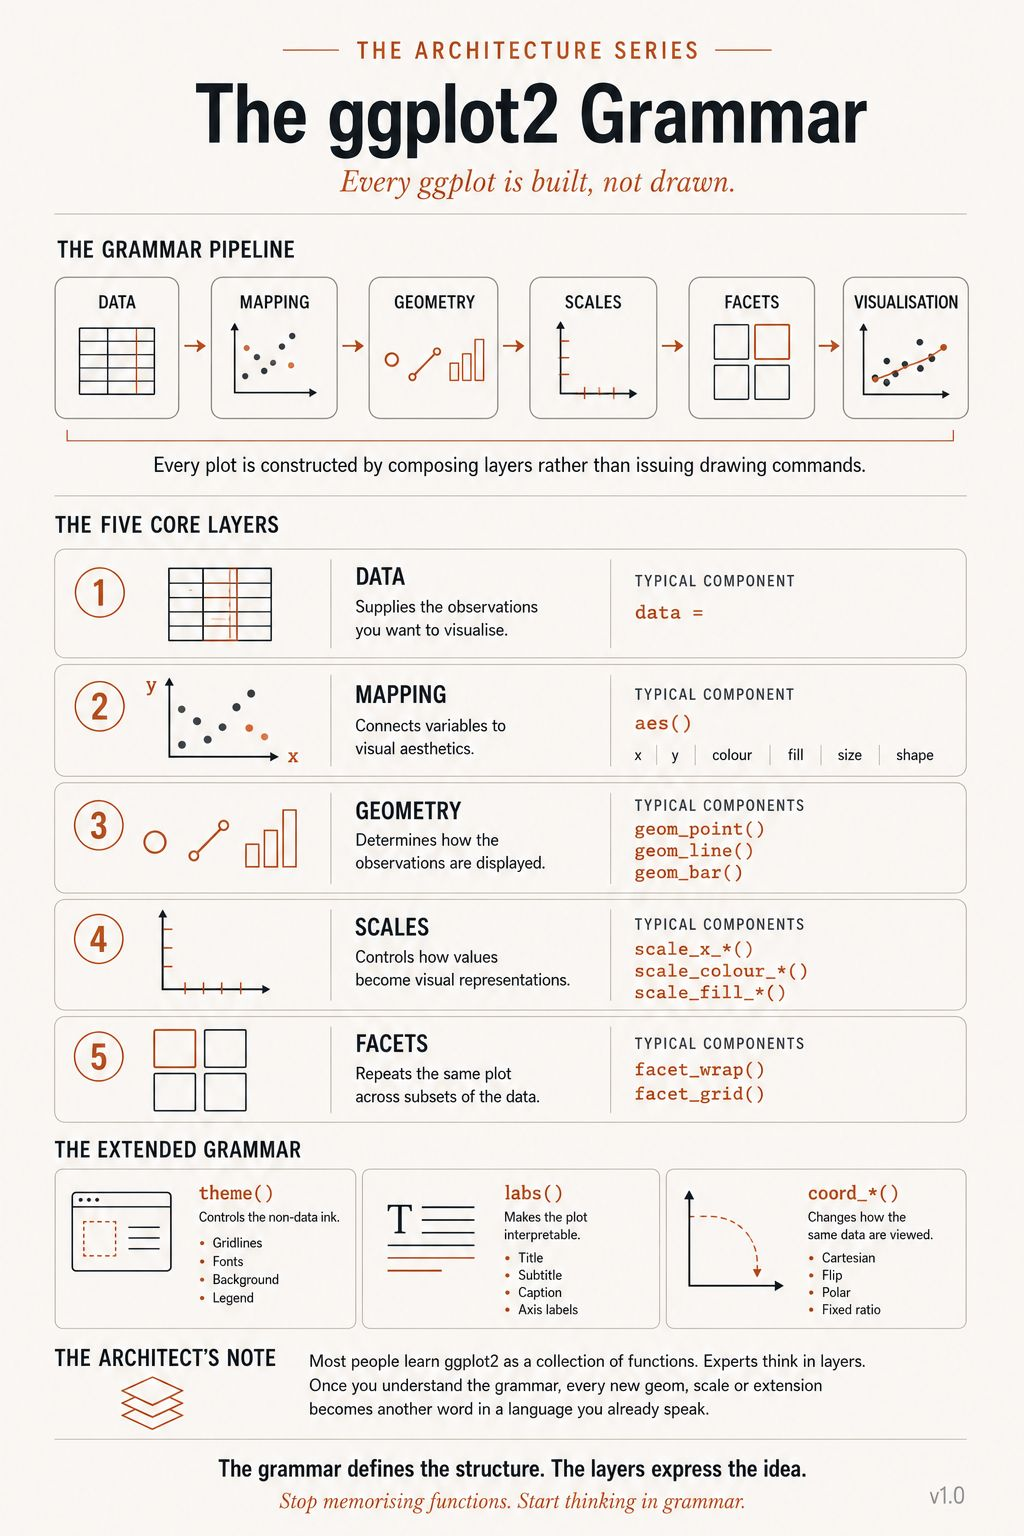
\includegraphics[width=\linewidth,height=6cm,keepaspectratio]{figures/ggplot2.jpg}
\end{center}

\normalsize

\centering

\begingroup \tiny source: \url{https://linkedin.com/in/adalbert-ngongang-phd-637995a3}\endgroup
\end{column}
\end{columns}
\end{frame}

\begin{frame}[fragile]{Geoms are the fundamental building blocks}
\protect\phantomsection\label{geoms-are-the-fundamental-building-blocks}
\footnotesize

\begin{Shaded}
\begin{Highlighting}[]
\NormalTok{species\_count }\SpecialCharTok{|\textgreater{}}
  \FunctionTok{mutate}\NormalTok{(}\AttributeTok{n\_visits =} \FunctionTok{factor}\NormalTok{(n\_visits)) }\SpecialCharTok{|\textgreater{}} 
  \FunctionTok{ggplot}\NormalTok{() }\SpecialCharTok{+}
    \FunctionTok{geom\_point}\NormalTok{(}\FunctionTok{aes}\NormalTok{(}\AttributeTok{y =}\NormalTok{ median\_elevation, }\AttributeTok{x =}\NormalTok{ n\_visits))}
\end{Highlighting}
\end{Shaded}

\begin{center}
\includegraphics[width=\linewidth,height=0.5\textheight,keepaspectratio]{Rintro_files/figure-beamer/unnamed-chunk-40-1.pdf}
\end{center}

\normalsize
\end{frame}

\begin{frame}[fragile]{Geoms are the fundamental building blocks}
\protect\phantomsection\label{geoms-are-the-fundamental-building-blocks-1}
\footnotesize

\begin{Shaded}
\begin{Highlighting}[]
\NormalTok{species\_count }\SpecialCharTok{|\textgreater{}}
  \FunctionTok{mutate}\NormalTok{(}\AttributeTok{n\_visits =} \FunctionTok{factor}\NormalTok{(n\_visits)) }\SpecialCharTok{|\textgreater{}} 
  \FunctionTok{ggplot}\NormalTok{() }\SpecialCharTok{+}
    \FunctionTok{geom\_boxplot}\NormalTok{(}\FunctionTok{aes}\NormalTok{(}\AttributeTok{y =}\NormalTok{ median\_elevation, }\AttributeTok{x =}\NormalTok{ n\_visits))}
\end{Highlighting}
\end{Shaded}

\begin{center}
\includegraphics[width=\linewidth,height=0.5\textheight,keepaspectratio]{Rintro_files/figure-beamer/unnamed-chunk-41-1.pdf}
\end{center}

\normalsize
\end{frame}

\begin{frame}{Practice 9}
\protect\phantomsection\label{practice-9}
\begin{enumerate}
\tightlist
\item
  check the possible geoms in the official ggplot2 cheat sheet
  (accessible via Help)
\item
  explore briefly
  \href{https://r-graph-gallery.com}{r-graph-gallery.com}
\end{enumerate}
\end{frame}

\begin{frame}[fragile]{Objects created with \{sf\} can be plotted using
\{ggplot2\} too}
\protect\phantomsection\label{objects-created-with-sf-can-be-plotted-using-ggplot2-too}
\footnotesize

\begin{Shaded}
\begin{Highlighting}[]
\NormalTok{species\_count\_sf }\SpecialCharTok{|\textgreater{}}
  \FunctionTok{filter}\NormalTok{(year }\SpecialCharTok{==} \DecValTok{2025}\NormalTok{) }\SpecialCharTok{|\textgreater{}}
  \FunctionTok{ggplot}\NormalTok{() }\SpecialCharTok{+}
    \FunctionTok{geom\_sf}\NormalTok{(}\FunctionTok{aes}\NormalTok{(}\AttributeTok{size =}\NormalTok{ n\_recorded\_species)) }\CommentTok{\# geometry = geometry is assumed}
\end{Highlighting}
\end{Shaded}

\begin{center}
\includegraphics[width=\linewidth,height=0.5\textheight,keepaspectratio]{Rintro_files/figure-beamer/unnamed-chunk-42-1.pdf}
\end{center}

\normalsize
\end{frame}

\begin{frame}[fragile]{Understanding aesthetic mappings}
\protect\phantomsection\label{understanding-aesthetic-mappings}
\begin{itemize}
\tightlist
\item
  \texttt{aes()} is used to defined how data connect to plotting
  elements via aesthetics
\item
  different geom expect different mandatory and optional aesthetics\\
  (see e.g.~\texttt{?geom\_point})
\end{itemize}

\pause

\vspace{0.5em}

\begin{itemize}
\tightlist
\item
  \texttt{aes()} is not the place to force colours, sizes, etc.; it only
  forces relationship:
\end{itemize}

\begin{block}{Bad}
\protect\phantomsection\label{bad}
\footnotesize

\begin{Shaded}
\begin{Highlighting}[]
\FunctionTok{ggplot}\NormalTok{(species\_count) }\SpecialCharTok{+}
  \FunctionTok{geom\_point}\NormalTok{(}\FunctionTok{aes}\NormalTok{(}\AttributeTok{y =}\NormalTok{ n\_recorded\_species, }\AttributeTok{x =}\NormalTok{ route\_length, }\AttributeTok{colour =} \StringTok{"blue"}\NormalTok{))}
\end{Highlighting}
\end{Shaded}

\normalsize
\end{block}

\begin{block}{Good}
\protect\phantomsection\label{good}
\footnotesize

\begin{Shaded}
\begin{Highlighting}[]
\FunctionTok{ggplot}\NormalTok{(species\_count) }\SpecialCharTok{+}
  \FunctionTok{geom\_point}\NormalTok{(}\FunctionTok{aes}\NormalTok{(}\AttributeTok{y =}\NormalTok{ n\_recorded\_species, }\AttributeTok{x =}\NormalTok{ route\_length), }\AttributeTok{colour =} \StringTok{"blue"}\NormalTok{)}
\end{Highlighting}
\end{Shaded}

\normalsize
\end{block}
\end{frame}

\begin{frame}[fragile]{Understanding aesthetic mappings}
\protect\phantomsection\label{understanding-aesthetic-mappings-1}
\begin{itemize}
\tightlist
\item
  \texttt{aes()} can be located outside a geom to apply to several of
  them at once:
\end{itemize}

\footnotesize

\begin{Shaded}
\begin{Highlighting}[]
\NormalTok{species\_count }\SpecialCharTok{|\textgreater{}}
    \FunctionTok{filter}\NormalTok{(year }\SpecialCharTok{==} \DecValTok{2025}\NormalTok{) }\SpecialCharTok{|\textgreater{}} 
    \FunctionTok{mutate}\NormalTok{(}\AttributeTok{n\_visits =} \FunctionTok{factor}\NormalTok{(n\_visits)) }\SpecialCharTok{|\textgreater{}} 
    \FunctionTok{ggplot}\NormalTok{(}\FunctionTok{aes}\NormalTok{(}\AttributeTok{y =}\NormalTok{ median\_elevation, }\AttributeTok{x =}\NormalTok{ n\_visits)) }\SpecialCharTok{+}
      \FunctionTok{geom\_violin}\NormalTok{() }\SpecialCharTok{+}
      \FunctionTok{geom\_jitter}\NormalTok{(}\AttributeTok{height =} \DecValTok{0}\NormalTok{, }\AttributeTok{width =} \FloatTok{0.1}\NormalTok{)}
\end{Highlighting}
\end{Shaded}

\begin{center}
\includegraphics[width=\linewidth,height=0.5\textheight,keepaspectratio]{Rintro_files/figure-beamer/unnamed-chunk-45-1.pdf}
\end{center}

\normalsize
\end{frame}

\begin{frame}[fragile]{Plot different subsets using faceting}
\protect\phantomsection\label{plot-different-subsets-using-faceting}
\footnotesize

\begin{Shaded}
\begin{Highlighting}[]
\NormalTok{species\_count\_sf }\SpecialCharTok{|\textgreater{}}
    \FunctionTok{mutate}\NormalTok{(}\AttributeTok{hotspot =} \FunctionTok{factor}\NormalTok{(n\_recorded\_species }\SpecialCharTok{\textgreater{}} \DecValTok{50}\NormalTok{)) }\SpecialCharTok{|\textgreater{}} 
    \FunctionTok{ggplot}\NormalTok{() }\SpecialCharTok{+}
      \FunctionTok{geom\_sf}\NormalTok{(}\FunctionTok{aes}\NormalTok{(}\AttributeTok{colour =}\NormalTok{ hotspot, }\AttributeTok{alpha =}\NormalTok{ hotspot)) }\SpecialCharTok{+}
      \FunctionTok{facet\_wrap}\NormalTok{(}\SpecialCharTok{\textasciitilde{}}\NormalTok{ year)}
\end{Highlighting}
\end{Shaded}

\begin{center}
\includegraphics[width=\linewidth,height=0.6\textheight,keepaspectratio]{Rintro_files/figure-beamer/unnamed-chunk-46-1.pdf}
\end{center}

\normalsize
\end{frame}

\begin{frame}[fragile]{Making plots beautiful \& readable}
\protect\phantomsection\label{making-plots-beautiful-readable}
Much can be achieved by using a better theme and defining scales:

\footnotesize

\begin{Shaded}
\begin{Highlighting}[]
\NormalTok{species\_count\_sf }\SpecialCharTok{|\textgreater{}}
    \FunctionTok{filter}\NormalTok{(year }\SpecialCharTok{==} \DecValTok{2025}\NormalTok{) }\SpecialCharTok{|\textgreater{}} 
    \FunctionTok{ggplot}\NormalTok{() }\SpecialCharTok{+}
        \FunctionTok{geom\_sf}\NormalTok{(}\FunctionTok{aes}\NormalTok{(}\AttributeTok{size =}\NormalTok{ n\_recorded\_species,}
                    \AttributeTok{colour =}\NormalTok{ n\_recorded\_species)) }\SpecialCharTok{+}
        \FunctionTok{scale\_color\_binned}\NormalTok{(}\AttributeTok{palette =}\NormalTok{ rainbow, }\AttributeTok{name =} \StringTok{"Nb. of species"}\NormalTok{) }\SpecialCharTok{+}
        \FunctionTok{scale\_size\_binned}\NormalTok{(}\AttributeTok{range =} \FunctionTok{c}\NormalTok{(}\FloatTok{0.5}\NormalTok{, }\DecValTok{5}\NormalTok{), }\AttributeTok{name =} \StringTok{"Nb. of species"}\NormalTok{) }\SpecialCharTok{+}
        \FunctionTok{guides}\NormalTok{(}\AttributeTok{size =} \FunctionTok{guide\_bins}\NormalTok{(), }\AttributeTok{color =} \FunctionTok{guide\_bins}\NormalTok{()) }\SpecialCharTok{+} \CommentTok{\# unusually needed here}
        \FunctionTok{theme\_bw}\NormalTok{(}\AttributeTok{base\_size =} \DecValTok{25}\NormalTok{)}
\end{Highlighting}
\end{Shaded}

\begin{center}
\includegraphics[width=\linewidth,height=0.3\textheight,keepaspectratio]{Rintro_files/figure-beamer/unnamed-chunk-47-1.pdf}
\end{center}

\normalsize
\end{frame}

\begin{frame}[fragile]{Making plots beautiful \& readable}
\protect\phantomsection\label{making-plots-beautiful-readable-1}
To modify the theme yourself, use \texttt{theme\_sub\_*()} or
(\texttt{theme()}) in combination with the appropriate
\texttt{element\_*()} function:

\footnotesize

\begin{Shaded}
\begin{Highlighting}[]
\FunctionTok{ggplot}\NormalTok{(species\_count) }\SpecialCharTok{+}
  \FunctionTok{geom\_point}\NormalTok{(}\FunctionTok{aes}\NormalTok{(}\AttributeTok{y =}\NormalTok{ n\_recorded\_species, }\AttributeTok{x =}\NormalTok{ route\_length)) }\SpecialCharTok{+}
  \FunctionTok{theme\_sub\_axis}\NormalTok{(}\AttributeTok{text =} \FunctionTok{element\_text}\NormalTok{(}\AttributeTok{size =} \DecValTok{15}\NormalTok{, }\AttributeTok{face =} \StringTok{"bold"}\NormalTok{, }\AttributeTok{colour =} \StringTok{"red"}\NormalTok{),}
                 \AttributeTok{title =} \FunctionTok{element\_text}\NormalTok{(}\AttributeTok{face =} \StringTok{"italic"}\NormalTok{, }\AttributeTok{hjust =} \DecValTok{1}\NormalTok{)) }\SpecialCharTok{+}
  \FunctionTok{theme\_sub\_panel}\NormalTok{(}\AttributeTok{grid.major.x =} \FunctionTok{element\_line}\NormalTok{(}\AttributeTok{linetype =} \StringTok{"dotted"}\NormalTok{, }\AttributeTok{colour =} \StringTok{"black"}\NormalTok{),}
                  \AttributeTok{background =} \FunctionTok{element\_rect}\NormalTok{(}\AttributeTok{fill =} \StringTok{"lightgreen"}\NormalTok{)) }\SpecialCharTok{+}
  \FunctionTok{theme\_sub\_plot}\NormalTok{(}\AttributeTok{background =} \FunctionTok{element\_rect}\NormalTok{(}\AttributeTok{fill =} \StringTok{"dodgerblue"}\NormalTok{, }\AttributeTok{colour =} \StringTok{"goldenrod"}\NormalTok{,}
                                           \AttributeTok{linewidth =} \DecValTok{10}\NormalTok{))}
\end{Highlighting}
\end{Shaded}

\begin{center}
\includegraphics[width=\linewidth,height=0.3\textheight,keepaspectratio]{Rintro_files/figure-beamer/unnamed-chunk-48-1.pdf}
\end{center}

\normalsize
\end{frame}

\begin{frame}[fragile]{Making plots beautiful \& readable}
\protect\phantomsection\label{making-plots-beautiful-readable-2}
You can define a common theme to be used for all your plots:

\footnotesize

\begin{Shaded}
\begin{Highlighting}[]
\NormalTok{(}\FunctionTok{theme\_bw}\NormalTok{(}\AttributeTok{base\_size =} \DecValTok{20}\NormalTok{) }\SpecialCharTok{+}
  \FunctionTok{theme\_sub\_axis}\NormalTok{(}\AttributeTok{text =} \FunctionTok{element\_text}\NormalTok{(}\AttributeTok{colour =} \StringTok{"red"}\NormalTok{))) }\SpecialCharTok{|\textgreater{}} 
  \FunctionTok{theme\_set}\NormalTok{()}

\FunctionTok{ggplot}\NormalTok{(species\_count) }\SpecialCharTok{+}
  \FunctionTok{geom\_point}\NormalTok{(}\FunctionTok{aes}\NormalTok{(}\AttributeTok{y =}\NormalTok{ n\_recorded\_species, }\AttributeTok{x =}\NormalTok{ route\_length))}
\end{Highlighting}
\end{Shaded}

\begin{center}
\includegraphics[width=\linewidth,height=0.4\textheight,keepaspectratio]{Rintro_files/figure-beamer/unnamed-chunk-49-1.pdf}
\end{center}

\normalsize

\textbf{NB:} the extra \texttt{()} are needed since
\texttt{\textbar{}\textgreater{}} binds more tightly than \texttt{+}
\end{frame}

\begin{frame}{Practice 10}
\protect\phantomsection\label{practice-10}
\begin{itemize}
\tightlist
\item
  combine data wrangling and plotting to illustrate the change in
  species abundance across years for the top 6 most encountered species
\end{itemize}
\end{frame}

\section{A dash of base R}\label{a-dash-of-base-r}

\begin{frame}[fragile]{What is base R?}
\protect\phantomsection\label{what-is-base-r}
\begin{block}{This is not base R (it relies on \{tidyverse\}, an
external R package)}
\protect\phantomsection\label{this-is-not-base-r-it-relies-on-tidyverse-an-external-r-package}
\footnotesize

\begin{Shaded}
\begin{Highlighting}[]
\NormalTok{species\_count }\SpecialCharTok{|\textgreater{}} 
    \FunctionTok{summarise}\NormalTok{(}\AttributeTok{mean\_nb\_sp =} \FunctionTok{mean}\NormalTok{(n\_recorded\_species), }\AttributeTok{.by =}\NormalTok{ year)}
\end{Highlighting}
\end{Shaded}

\begin{verbatim}
# A tibble: 27 x 2
   year mean_nb_sp
  <dbl>      <dbl>
1  1999       31.4
2  2000       32.5
3  2001       32.7
# i 24 more rows
\end{verbatim}

\normalsize
\end{block}
\end{frame}

\begin{frame}[fragile]{What is base R?}
\protect\phantomsection\label{what-is-base-r-1}
\begin{block}{This is typical base R (it does not rely on an external R
package)}
\protect\phantomsection\label{this-is-typical-base-r-it-does-not-rely-on-an-external-r-package}
\footnotesize

\begin{Shaded}
\begin{Highlighting}[]
\NormalTok{results }\OtherTok{\textless{}{-}} \FunctionTok{data.frame}\NormalTok{(}\AttributeTok{year =} \FunctionTok{unique}\NormalTok{(species\_count}\SpecialCharTok{$}\NormalTok{year), }\AttributeTok{mean\_nb\_sp =} \ConstantTok{NA}\NormalTok{)}
\ControlFlowTok{for}\NormalTok{ (y }\ControlFlowTok{in} \FunctionTok{unique}\NormalTok{(species\_count}\SpecialCharTok{$}\NormalTok{year)) \{}
\NormalTok{    n\_recorded\_species\_year }\OtherTok{\textless{}{-}}\NormalTok{ species\_count}\SpecialCharTok{$}\NormalTok{n\_recorded\_species[species\_count}\SpecialCharTok{$}\NormalTok{year }\SpecialCharTok{==}\NormalTok{ y]}
\NormalTok{    results[results}\SpecialCharTok{$}\NormalTok{year }\SpecialCharTok{==}\NormalTok{ y, }\StringTok{"mean\_nb\_sp"}\NormalTok{] }\OtherTok{\textless{}{-}} \FunctionTok{mean}\NormalTok{(n\_recorded\_species\_year)}
\NormalTok{\}}
\FunctionTok{head}\NormalTok{(results, }\AttributeTok{n =} \DecValTok{3}\NormalTok{)}
\end{Highlighting}
\end{Shaded}

\begin{verbatim}
  year mean_nb_sp
1 1999   31.36515
2 2000   32.48485
3 2001   32.70270
\end{verbatim}

\normalsize

\vspace{1em}

\textbf{NB:}

\begin{itemize}
\tightlist
\item
  it looks more complicated (but from a developer's perspective, it is
  actually clearer)
\end{itemize}
\end{block}
\end{frame}

\begin{frame}[fragile]{What is base R?}
\protect\phantomsection\label{what-is-base-r-2}
\begin{block}{But this is also base R (and a little closer to
\{tidyverse\} in spirit)}
\protect\phantomsection\label{but-this-is-also-base-r-and-a-little-closer-to-tidyverse-in-spirit}
\footnotesize

\begin{Shaded}
\begin{Highlighting}[]
\NormalTok{results }\OtherTok{\textless{}{-}} \FunctionTok{with}\NormalTok{(species\_count, }
                \FunctionTok{aggregate}\NormalTok{(}\FunctionTok{list}\NormalTok{(}\AttributeTok{mean\_nb\_sp =}\NormalTok{ n\_recorded\_species),}
                          \AttributeTok{by =} \FunctionTok{list}\NormalTok{(}\AttributeTok{year =}\NormalTok{ year), }\AttributeTok{FUN =}\NormalTok{ mean))}
\FunctionTok{head}\NormalTok{(results, }\AttributeTok{n =} \DecValTok{3}\NormalTok{)}
\end{Highlighting}
\end{Shaded}

\begin{verbatim}
  year mean_nb_sp
1 1999   31.36515
2 2000   32.48485
3 2001   32.70270
\end{verbatim}

\normalsize

\vspace{1em}

\textbf{NB:}

\begin{itemize}
\tightlist
\item
  there are often plenty of alternatives to achieve the same output
\end{itemize}
\end{block}
\end{frame}

\begin{frame}{Some key objects in base R}
\protect\phantomsection\label{some-key-objects-in-base-r}
\tiny

{\def\LTcaptype{none} % do not increment counter
\begin{longtable}[]{@{}
  >{\raggedright\arraybackslash}p{(\linewidth - 6\tabcolsep) * \real{0.1694}}
  >{\centering\arraybackslash}p{(\linewidth - 6\tabcolsep) * \real{0.2419}}
  >{\raggedright\arraybackslash}p{(\linewidth - 6\tabcolsep) * \real{0.3306}}
  >{\raggedright\arraybackslash}p{(\linewidth - 6\tabcolsep) * \real{0.2581}}@{}}
\toprule\noalign{}
\begin{minipage}[b]{\linewidth}\raggedright
object
\end{minipage} & \begin{minipage}[b]{\linewidth}\centering
typical number of dimensions
\end{minipage} & \begin{minipage}[b]{\linewidth}\raggedright
content restriction
\end{minipage} & \begin{minipage}[b]{\linewidth}\raggedright
usage example
\end{minipage} \\
\midrule\noalign{}
\endhead
the \blueit{vector} & 1 & all elements must have same type & storing
data for a variable \\
the \blueit{list} & tree-like structure & each list can be anything &
output of model fit \\
the \blueit{matrix} & 2 & elements must have same type everywhere &
design matrix of a linear model \\
the \blueit{array} & N & elements must have same type everywhere &
posteriors in Bayesian analyses \\
the \blueit{data frame} or \blueit{tibble} & 2 & elements must have same
type in a column & input data for a model \\
\bottomrule\noalign{}
\end{longtable}
}

\vspace{1em}

\pause

\small

\textbf{NB:}

\begin{itemize}
\tightlist
\item
  the different objects are generally created by functions, so you won't
  have to worry about creating them
\item
  what you need to worry about is how to extract information from each
  of those objects
\end{itemize}
\end{frame}

\begin{frame}[fragile]{Extracting elements from vectors}
\protect\phantomsection\label{extracting-elements-from-vectors}
\footnotesize

\begin{Shaded}
\begin{Highlighting}[]
\NormalTok{some\_vector }\OtherTok{\textless{}{-}}\NormalTok{ letters }\CommentTok{\# we create a small vector}
\NormalTok{some\_vector}
\end{Highlighting}
\end{Shaded}

\begin{verbatim}
 [1] "a" "b" "c" "d" "e" "f" "g" "h" "i" "j" "k" "l" "m" "n" "o" "p" "q" "r" "s" "t" "u"
[22] "v" "w" "x" "y" "z"
\end{verbatim}

\begin{Shaded}
\begin{Highlighting}[]
\NormalTok{some\_vector[}\FunctionTok{c}\NormalTok{(}\DecValTok{1}\NormalTok{, }\DecValTok{12}\NormalTok{, }\DecValTok{5}\NormalTok{, }\DecValTok{24}\NormalTok{)]}
\end{Highlighting}
\end{Shaded}

\begin{verbatim}
[1] "a" "l" "e" "x"
\end{verbatim}

\begin{Shaded}
\begin{Highlighting}[]
\NormalTok{some\_vector[some\_vector }\SpecialCharTok{\%in\%} \FunctionTok{c}\NormalTok{(}\StringTok{"a"}\NormalTok{, }\StringTok{"l"}\NormalTok{, }\StringTok{"e"}\NormalTok{, }\StringTok{"x"}\NormalTok{)]}
\end{Highlighting}
\end{Shaded}

\begin{verbatim}
[1] "a" "e" "l" "x"
\end{verbatim}

\begin{Shaded}
\begin{Highlighting}[]
\NormalTok{some\_namedvector }\OtherTok{\textless{}{-}} \FunctionTok{c}\NormalTok{(}\AttributeTok{a =} \DecValTok{1}\NormalTok{, }\AttributeTok{b =} \DecValTok{5}\NormalTok{)}
\NormalTok{some\_namedvector[}\StringTok{"b"}\NormalTok{]}
\end{Highlighting}
\end{Shaded}

\begin{verbatim}
b 
5 
\end{verbatim}

\normalsize
\end{frame}

\begin{frame}[fragile]{Extracting elements from lists}
\protect\phantomsection\label{extracting-elements-from-lists}
\footnotesize

\begin{Shaded}
\begin{Highlighting}[]
\NormalTok{some\_list }\OtherTok{\textless{}{-}} \FunctionTok{list}\NormalTok{(}\DecValTok{1}\NormalTok{, }\DecValTok{1}\SpecialCharTok{:}\DecValTok{5}\NormalTok{) }\CommentTok{\# we create a small list}
\NormalTok{some\_list}
\end{Highlighting}
\end{Shaded}

\begin{verbatim}
[[1]]
[1] 1

[[2]]
[1] 1 2 3 4 5
\end{verbatim}

\begin{Shaded}
\begin{Highlighting}[]
\NormalTok{some\_list[}\DecValTok{2}\NormalTok{]}
\end{Highlighting}
\end{Shaded}

\begin{verbatim}
[[1]]
[1] 1 2 3 4 5
\end{verbatim}

\begin{Shaded}
\begin{Highlighting}[]
\NormalTok{some\_list[[}\DecValTok{2}\NormalTok{]]}
\end{Highlighting}
\end{Shaded}

\begin{verbatim}
[1] 1 2 3 4 5
\end{verbatim}

\begin{Shaded}
\begin{Highlighting}[]
\NormalTok{some\_list[[}\DecValTok{2}\NormalTok{]][}\DecValTok{2}\NormalTok{]}
\end{Highlighting}
\end{Shaded}

\begin{verbatim}
[1] 2
\end{verbatim}

\normalsize
\end{frame}

\begin{frame}[fragile]{Extracting elements from named lists}
\protect\phantomsection\label{extracting-elements-from-named-lists}
\footnotesize

\begin{Shaded}
\begin{Highlighting}[]
\NormalTok{some\_namedlist }\OtherTok{\textless{}{-}} \FunctionTok{list}\NormalTok{(}\AttributeTok{a =} \DecValTok{1}\NormalTok{, }\AttributeTok{b =} \DecValTok{1}\SpecialCharTok{:}\DecValTok{5}\NormalTok{)}\CommentTok{\# we create a small named list}
\NormalTok{some\_namedlist[}\StringTok{"b"}\NormalTok{]}
\end{Highlighting}
\end{Shaded}

\begin{verbatim}
$b
[1] 1 2 3 4 5
\end{verbatim}

\begin{Shaded}
\begin{Highlighting}[]
\NormalTok{some\_namedlist[[}\StringTok{"b"}\NormalTok{]]}
\end{Highlighting}
\end{Shaded}

\begin{verbatim}
[1] 1 2 3 4 5
\end{verbatim}

\begin{Shaded}
\begin{Highlighting}[]
\NormalTok{some\_namedlist}\SpecialCharTok{$}\NormalTok{b}
\end{Highlighting}
\end{Shaded}

\begin{verbatim}
[1] 1 2 3 4 5
\end{verbatim}

\normalsize
\end{frame}

\begin{frame}[fragile]{Extracting elements from matrices}
\protect\phantomsection\label{extracting-elements-from-matrices}
\footnotesize

\begin{Shaded}
\begin{Highlighting}[]
\NormalTok{some\_matrix }\OtherTok{\textless{}{-}} \FunctionTok{matrix}\NormalTok{(}\DecValTok{1}\SpecialCharTok{:}\DecValTok{9}\NormalTok{, }\AttributeTok{nrow =} \DecValTok{3}\NormalTok{) }\CommentTok{\# we create a small matrix}
\NormalTok{some\_matrix}
\end{Highlighting}
\end{Shaded}

\begin{verbatim}
     [,1] [,2] [,3]
[1,]    1    4    7
[2,]    2    5    8
[3,]    3    6    9
\end{verbatim}

\begin{Shaded}
\begin{Highlighting}[]
\NormalTok{some\_matrix[}\DecValTok{2}\NormalTok{, ]}
\end{Highlighting}
\end{Shaded}

\begin{verbatim}
[1] 2 5 8
\end{verbatim}

\begin{Shaded}
\begin{Highlighting}[]
\NormalTok{some\_matrix[, }\DecValTok{2}\NormalTok{]}
\end{Highlighting}
\end{Shaded}

\begin{verbatim}
[1] 4 5 6
\end{verbatim}

\begin{Shaded}
\begin{Highlighting}[]
\NormalTok{some\_matrix[}\DecValTok{2}\NormalTok{, }\DecValTok{2}\NormalTok{]}
\end{Highlighting}
\end{Shaded}

\begin{verbatim}
[1] 5
\end{verbatim}

\normalsize
\end{frame}

\begin{frame}[fragile]{Extracting elements from matrices}
\protect\phantomsection\label{extracting-elements-from-matrices-1}
\footnotesize

\begin{Shaded}
\begin{Highlighting}[]
\NormalTok{some\_matrix[}\FunctionTok{c}\NormalTok{(}\DecValTok{1}\NormalTok{, }\DecValTok{3}\NormalTok{), }\FunctionTok{c}\NormalTok{(}\DecValTok{1}\NormalTok{, }\DecValTok{3}\NormalTok{)]}
\end{Highlighting}
\end{Shaded}

\begin{verbatim}
     [,1] [,2]
[1,]    1    7
[2,]    3    9
\end{verbatim}

\begin{Shaded}
\begin{Highlighting}[]
\NormalTok{some\_matrix[}\FunctionTok{cbind}\NormalTok{(}\FunctionTok{c}\NormalTok{(}\DecValTok{1}\NormalTok{, }\DecValTok{3}\NormalTok{), }\FunctionTok{c}\NormalTok{(}\DecValTok{1}\NormalTok{, }\DecValTok{3}\NormalTok{))]}
\end{Highlighting}
\end{Shaded}

\begin{verbatim}
[1] 1 9
\end{verbatim}

\normalsize
\end{frame}

\begin{frame}[fragile]{Extracting elements from named matrices}
\protect\phantomsection\label{extracting-elements-from-named-matrices}
\footnotesize

\begin{Shaded}
\begin{Highlighting}[]
\FunctionTok{colnames}\NormalTok{(some\_matrix) }\OtherTok{\textless{}{-}} \FunctionTok{paste0}\NormalTok{(}\StringTok{"col\_"}\NormalTok{, }\DecValTok{1}\SpecialCharTok{:}\DecValTok{3}\NormalTok{) }\CommentTok{\# we name the columns}
\FunctionTok{rownames}\NormalTok{(some\_matrix) }\OtherTok{\textless{}{-}} \FunctionTok{paste0}\NormalTok{(}\StringTok{"row\_"}\NormalTok{, }\DecValTok{1}\SpecialCharTok{:}\DecValTok{3}\NormalTok{) }\CommentTok{\# we name the rows}
\NormalTok{some\_matrix}
\end{Highlighting}
\end{Shaded}

\begin{verbatim}
      col_1 col_2 col_3
row_1     1     4     7
row_2     2     5     8
row_3     3     6     9
\end{verbatim}

\begin{Shaded}
\begin{Highlighting}[]
\NormalTok{some\_matrix[}\StringTok{"row\_2"}\NormalTok{, }\StringTok{"col\_3"}\NormalTok{]}
\end{Highlighting}
\end{Shaded}

\begin{verbatim}
[1] 8
\end{verbatim}

\normalsize
\end{frame}

\begin{frame}[fragile]{Extracting elements from arrays}
\protect\phantomsection\label{extracting-elements-from-arrays}
\footnotesize

\begin{Shaded}
\begin{Highlighting}[]
\NormalTok{some\_array }\OtherTok{\textless{}{-}} \FunctionTok{array}\NormalTok{(}\DecValTok{1}\SpecialCharTok{:}\DecValTok{30}\NormalTok{, }\AttributeTok{dim =} \FunctionTok{c}\NormalTok{(}\DecValTok{5}\NormalTok{, }\DecValTok{3}\NormalTok{, }\DecValTok{2}\NormalTok{)) }\CommentTok{\# we create a small 3D array}
\end{Highlighting}
\end{Shaded}

\normalsize

\begin{columns}[T]
\begin{column}{0.33\linewidth}
\scriptsize

\begin{Shaded}
\begin{Highlighting}[]
\NormalTok{some\_array}
\end{Highlighting}
\end{Shaded}

\begin{verbatim}
, , 1

     [,1] [,2] [,3]
[1,]    1    6   11
[2,]    2    7   12
[3,]    3    8   13
[4,]    4    9   14
[5,]    5   10   15

, , 2

     [,1] [,2] [,3]
[1,]   16   21   26
[2,]   17   22   27
[3,]   18   23   28
[4,]   19   24   29
[5,]   20   25   30
\end{verbatim}

\normalsize
\end{column}

\begin{column}{0.33\linewidth}
\scriptsize

\begin{Shaded}
\begin{Highlighting}[]
\NormalTok{some\_array[}\DecValTok{2}\NormalTok{, , ] }\CommentTok{\# rows}
\end{Highlighting}
\end{Shaded}

\begin{verbatim}
     [,1] [,2]
[1,]    2   17
[2,]    7   22
[3,]   12   27
\end{verbatim}

\normalsize
\vspace{1em}

\scriptsize

\begin{Shaded}
\begin{Highlighting}[]
\NormalTok{some\_array[, }\DecValTok{2}\NormalTok{, ] }\CommentTok{\# columns}
\end{Highlighting}
\end{Shaded}

\begin{verbatim}
     [,1] [,2]
[1,]    6   21
[2,]    7   22
[3,]    8   23
[4,]    9   24
[5,]   10   25
\end{verbatim}

\normalsize
\end{column}

\begin{column}{0.33\linewidth}
\scriptsize

\begin{Shaded}
\begin{Highlighting}[]
\NormalTok{some\_array[, , }\DecValTok{2}\NormalTok{] }\CommentTok{\# depth}
\end{Highlighting}
\end{Shaded}

\begin{verbatim}
     [,1] [,2] [,3]
[1,]   16   21   26
[2,]   17   22   27
[3,]   18   23   28
[4,]   19   24   29
[5,]   20   25   30
\end{verbatim}

\normalsize
\vspace{1em}

\scriptsize

\begin{Shaded}
\begin{Highlighting}[]
\NormalTok{some\_array[}\DecValTok{2}\NormalTok{, }\DecValTok{2}\NormalTok{, }\DecValTok{2}\NormalTok{] }\CommentTok{\# cell}
\end{Highlighting}
\end{Shaded}

\begin{verbatim}
[1] 22
\end{verbatim}

\normalsize
\vspace{1em}

\scriptsize

\begin{Shaded}
\begin{Highlighting}[]
\NormalTok{some\_array[}\DecValTok{2}\NormalTok{, , }\DecValTok{2}\NormalTok{] }\CommentTok{\# row 2}
                   \CommentTok{\# at depth 2}
\end{Highlighting}
\end{Shaded}

\begin{verbatim}
[1] 17 22 27
\end{verbatim}

\normalsize
\end{column}
\end{columns}
\end{frame}

\begin{frame}[fragile]{Extracting elements from data frames / tibbles}
\protect\phantomsection\label{extracting-elements-from-data-frames-tibbles}
\footnotesize

\begin{Shaded}
\begin{Highlighting}[]
\NormalTok{species\_count[}\DecValTok{1}\NormalTok{, ]}
\end{Highlighting}
\end{Shaded}

\begin{verbatim}
# A tibble: 1 x 10
  samplearea_id `x-koord` `y-koord`   lon   lat  year route_length median_elevation
          <dbl>     <dbl>     <dbl> <dbl> <dbl> <dbl>        <dbl>            <dbl>
1           268   2725500   1182500  9.08  46.8  1999         4444             1550
# i 2 more variables: n_visits <dbl>, n_recorded_species <dbl>
\end{verbatim}

\begin{Shaded}
\begin{Highlighting}[]
\NormalTok{species\_count[, }\DecValTok{1}\NormalTok{]}
\end{Highlighting}
\end{Shaded}

\begin{verbatim}
# A tibble: 7,113 x 1
  samplearea_id
          <dbl>
1           268
2           268
3           268
# i 7,110 more rows
\end{verbatim}

\normalsize
\end{frame}

\begin{frame}[fragile]{Extracting elements from data frames / tibbles}
\protect\phantomsection\label{extracting-elements-from-data-frames-tibbles-1}
\footnotesize

\begin{Shaded}
\begin{Highlighting}[]
\NormalTok{species\_count[, }\StringTok{"year"}\NormalTok{]}
\end{Highlighting}
\end{Shaded}

\begin{verbatim}
# A tibble: 7,113 x 1
   year
  <dbl>
1  1999
2  2000
3  2001
# i 7,110 more rows
\end{verbatim}

\begin{Shaded}
\begin{Highlighting}[]
\NormalTok{species\_count[}\StringTok{"year"}\NormalTok{]}
\end{Highlighting}
\end{Shaded}

\begin{verbatim}
# A tibble: 7,113 x 1
   year
  <dbl>
1  1999
2  2000
3  2001
# i 7,110 more rows
\end{verbatim}

\normalsize
\end{frame}

\begin{frame}[fragile]{Extracting elements from data frames / tibbles}
\protect\phantomsection\label{extracting-elements-from-data-frames-tibbles-2}
\footnotesize

\begin{Shaded}
\begin{Highlighting}[]
\NormalTok{species\_count\_small }\OtherTok{\textless{}{-}} \FunctionTok{slice}\NormalTok{(species\_count, }\DecValTok{1}\SpecialCharTok{:}\DecValTok{10}\NormalTok{) }\CommentTok{\# for smaller data}
\NormalTok{species\_count\_small[[}\StringTok{"year"}\NormalTok{]]}
\end{Highlighting}
\end{Shaded}

\begin{verbatim}
 [1] 1999 2000 2001 2002 2003 2004 2005 2006 2007 2008
\end{verbatim}

\begin{Shaded}
\begin{Highlighting}[]
\NormalTok{species\_count\_small}\SpecialCharTok{$}\NormalTok{year}
\end{Highlighting}
\end{Shaded}

\begin{verbatim}
 [1] 1999 2000 2001 2002 2003 2004 2005 2006 2007 2008
\end{verbatim}

\normalsize
\end{frame}

\begin{frame}[fragile]{A few very useful base R functions I would be sad
to work without}
\protect\phantomsection\label{a-few-very-useful-base-r-functions-i-would-be-sad-to-work-without}
Check the following on your own time:

\begin{itemize}
\tightlist
\item
  \texttt{help()} for help (or \texttt{?} for short)
\item
  \texttt{plot()} for fast \& dirty plots
\item
  \texttt{str()} for inspecting objects
\item
  \texttt{dput()} for sharing a reproducible example when asking for
  help (useful for LLMs)
\item
  \texttt{function()} for creating a function (or
  \texttt{\textbackslash{}()} for short)
\item
  \texttt{debugonce()} for debugging a function line by line
\item
  \texttt{rnorm()}, \texttt{runif()} for simulating data
\item
  \texttt{set.seed()} for ``fixing'' randomness
\item
  \texttt{replicate()} for doing something several times
\end{itemize}

\textbf{Pro tips:}

\begin{itemize}
\tightlist
\item
  check them out in your own time; they are worth learning about
\end{itemize}
\end{frame}

\section{House keeping}\label{house-keeping}

\begin{frame}{When and what to update}
\protect\phantomsection\label{when-and-what-to-update}
\begin{itemize}
\tightlist
\item
  update R packages regularly using the RStudio ``Packages tab''\\
  (at least once a month)
\item
  update R a few times a year:\\
  check \href{https://www.r-project.org}{www.r-project.org} (May and
  October tend to be good times)
\item
  update RStudio at least after each update of R
\end{itemize}
\end{frame}

\section{Learning more}\label{learning-more}

\begin{frame}{Getting help}
\protect\phantomsection\label{getting-help}
\begin{itemize}
\tightlist
\item
  don't forget that functions have help pages associated to them
\item
  R for Data Science free book:
  \href{https://r4ds.hadley.nz}{r4ds.hadley.nz}
\item
  there is an active Slack channel: \href{https://dslc.io}{dslc.io}
\item
  talk to each other
\item
  LLMs?\\
  if you do, don't blindly copy/paste, and beware:\\
  LLMs make mistakes and make things up
\end{itemize}
\end{frame}

\begin{frame}{Getting better}
\protect\phantomsection\label{getting-better}
\begin{itemize}
\tightlist
\item
  learn ``base R'' too
  (e.g.~\href{https://cran.r-project.org/doc/manuals/r-release/R-intro.html}{cran.r-project.org/doc/manuals/r-release/R-intro.html})
\item
  try to understand why things do not behave as you expect by
  experimenting \&\\
  avoid always using a workaround
\item
  do use LLMs to review your code (rather than to create it)\\
  the more you know, the more LLMs will be helpful to you!
\end{itemize}
\end{frame}

\section*{Questions?}\label{questions}




\end{document}
